% !Mode:: "TeX:UTF-8"
% 2026 APMCM Problem C -- full paper
% Compile with: xelatex main.tex  (run twice for the table of contents)
\documentclass{apmcmthesis}
\renewcommand*{\baselinestretch}{1.15}
\geometry{top=24mm,bottom=24mm,left=25mm,right=25mm}

\usepackage{url}
\usepackage[hidelinks]{hyperref}

\newcommand{\R}{\mathbb{R}}
\newcommand{\E}{\mathbb{E}}
\newcommand{\Prob}{\mathbb{P}}

\graphicspath{{./}}
\setlength{\emergencystretch}{1.5em}

\titleformat{\section}{\centering\normalfont\Large\bfseries}{\thesection.}{.5em}{}

%%%%%%%%%%%% 相关信息 %%%%%%%%%%%%%%%%%%%%%%%%%%
\tihao{C}
\baominghao{apmcm263XXXXX}
%%%%%%%%%%%%%%%%%%%%%%%%%%%%%%%%%%%%%%%%%%%%%%%%



\begin{document}
\pagestyle{frontmatterstyle}

\begin{abstract}
African penguins (\textit{Spheniscus demersus}) are critically endangered and depend on
acoustic contact at sea to maintain group cohesion and to recruit conspecifics to foraging
aggregations. We integrate three datasets supplied with the problem --- acoustic measurements
of 108 sea-surface calls (44 flat, 40 modulated, 24 two-voice), 278 playback trials organised
as 139 paired call--control experiments, and propagation correlations at seven distances from
4 to 256 m --- into a single chain that runs from signal structure to conservation advice.

For the acoustic question we show that the three call types differ mainly along the frequency
axis: peak frequency separates the groups after Holm correction ($H=12.28$, $p=0.013$), whereas
duration, Q25 and Q75 do not. A classifier restricted to the six shared acoustic features
reaches only a macro-$F_1$ of 0.458, and 0.952 when the structural indicators (presence of a
second fundamental, presence of a pulse rate) are admitted; the difference is label leakage,
not acoustic information.

For the propagation question we fuse spectrogram, amplitude-spectrum and envelope correlations
into a composite fidelity $F(d)$. Fidelity is nearly flat to 32 m and collapses between 64 and
256 m. At the operational threshold $\tau=0.5$ the effective ranges are 84.7 m (flat),
144.6 m (modulated) and 169.7 m (two-voice) under an equal-weight scheme, but the ranking is
model-dependent: a four-parameter Weibull reverses the modulated/two-voice order.

For the behavioural question we exploit the paired design. Natural calls raise the response
rate from 12.9\% to 64.8\% (McNemar OR $=37.0$, 95\% CI 9.9--311). In a GEE with experiment-level
clustering, call type (OR 13.7--22.4 versus control), distance (OR 0.49 per $e$-fold, $p=0.008$)
and group size (OR 0.94 per bird, $p=0.0045$) are associated with response; context is not after
adjustment. The distribution of the eight response combinations changes under playback
(paired permutation $p=0.0002$), and time to first response has a median of about 2 s with a
distance multiplier of 1.27 per $e$-fold.

For the conservation question we define the Communication Effectiveness Index
$\mathrm{CEI}(d)=F(d)\times P_{\mathrm{recruit}}(d)$, a product of two necessary conditions rather
than a compensable weighted sum. Its half-effectiveness radii are 137 m (flat), 175 m (modulated)
and 203 m (two-voice) empirically, with the two-voice value falling to 158 m under a logistic fit.
Recruitment probability declines only weakly with distance (OR 0.87 per $e$-fold, $p=0.59$), so
the radius is driven by fidelity; a 3 dB-equivalent fidelity loss would reduce the radii to
102--171 m. We translate the index into a
precautionary 200 m noise-management buffer with a 3 dB limit in the 0.5--2 kHz band, and we state
explicitly what the data cannot support: no response is not the same as no perception, and the
absence of a call-type effect on specific combinations is a power limitation, not evidence of
equivalence.

\keywords{acoustic communication \quad paired playback design \quad censored latency \quad composite fidelity \quad communication effectiveness index}
\end{abstract}

\newpage
\setcounter{tocdepth}{1}
\tableofcontents

\newpage
\pagestyle{mainmatterstyle}
\setcounter{page}{1}

\section{Introduction}

\subsection{Background}

The African penguin (\textit{Spheniscus demersus}) is listed as critically endangered, and its
population decline has been linked to the spatial mismatch between breeding colonies and the
location of prey. At sea, penguins forage in groups and appear to use vocal signals to maintain
contact, coordinate diving and recruit conspecifics to feeding aggregations. Unlike visual or
chemical signals, sound propagates over hundreds of metres in the shallow coastal water where
these birds forage, which makes acoustics the plausible channel for group-level coordination.
A conservation programme that wishes to reduce acoustic disturbance therefore needs three
quantities that connect to one another \cite{ref1,ref2,ref3}: the acoustic structure that carries identity and
intent, the physical distance over which that structure survives, and the behavioural
probability that a bird responds once the signal is audible.

The problem supplies exactly these three pieces of evidence, but not their connection.
Acoustic measurements describe what the calls look like; propagation recordings describe how
the signal degrades with distance; playback experiments describe how often penguins react.
Modelling the connection is not a matter of stacking three models. It requires deciding what
counts as ``hearing'', what counts as ``responding'', and how the two should be combined so
that the result can be used to size a protected buffer.

\subsection{Problem restatement}

We are asked to answer four linked questions.

\begin{enumerate}[leftmargin=1.6em,itemsep=2pt]
  \item Characterise the three call types (flat, modulated, two-voice) using the supplied
        acoustic measurements; identify which features separate them; build a classifier and
        use at least two nonparametric tests; and name the key acoustic indicators that later
        questions should carry forward.
  \item Fuse the three propagation correlations into a fidelity measure that varies with
        distance; fit degradation models for each call type; define a graded threshold scheme;
        estimate the effective communication range under two criteria, with uncertainty ranges;
        and conduct sensitivity analyses over thresholds, weights and model families.
  \item Analyse the playback experiments: compare natural calls with controls, relate response
        to context, call type, distance and group size within one modelling framework,
        describe the distribution of the eight possible response combinations, model response
        latency, and produce a numerical table for representative conditions.
  \item Combine fidelity and recruitment probability into a single communication-effectiveness
        index; state its functional form and the ecological interpretation of its weights; use
        it to estimate an effective radius or an expected number of responders; and translate
        the result into conservation recommendations together with the limitations of the data.
\end{enumerate}

\subsection{Approach and contributions}

Our approach follows the causal chain rather than the questionnaire. The contributions we claim
are the following.

\begin{itemize}[leftmargin=1.6em,itemsep=2pt]
  \item \textbf{We treat the playback experiment as a paired design throughout.} The 139
        experiments each contain one natural call and one control under the same date and
        context. Analyses that ignore this structure underestimate the call effect by a factor
        of nearly three (OR 12.4 instead of 37.0) and can make the distance effect disappear
        entirely. Every inferential statement in Section~\ref{sec:q3} is therefore built on
        within-pair contrasts or on clustered estimating equations.
  \item \textbf{We separate physical audibility from behavioural recruitment.} The fidelity
        index $F(d)$ answers ``is the signal still recognisable''; the recruitment probability
        $P_{\mathrm{recruit}}(d)$ answers ``will a bird come''. Their product, not their weighted
        sum, is the quantity a manager needs, because a signal that cannot be heard cannot
        recruit and a signal that is heard need not recruit. This is the index of Section~\ref{sec:q4}.
  \item \textbf{We model non-response as censoring rather than as a zero.} The problem states
        explicitly that no response does not mean no perception. We therefore split the analysis
        into a response probability and a latency model, carry non-responders as right-censored
        observations in the Kaplan--Meier summary, and report both a conditional median (among
        responders) and a restricted mean survival time that keeps non-responders in the
        denominator.
  \item \textbf{We report ranges instead of point values wherever the data support more than
        one defensible model.} Three of the seven analytic choices we examine --- the weight on
        the envelope correlation, the recognition threshold and the family of the decay curve ---
        each move the estimated radius by tens of metres, and in one case reverse the ranking of
        call types. Reporting a single ``true'' radius would misrepresent what is known.
\end{itemize}

Section~\ref{sec:data} describes the data and the assumptions that the rest of the paper depends
on. Sections~\ref{sec:q1}--\ref{sec:q4} answer the four problems. Section~\ref{sec:discussion}
collects the uncertainty analysis and the limitations, and Section~\ref{sec:conclusion} concludes.

\begin{figure}[htbp]
  \centering
  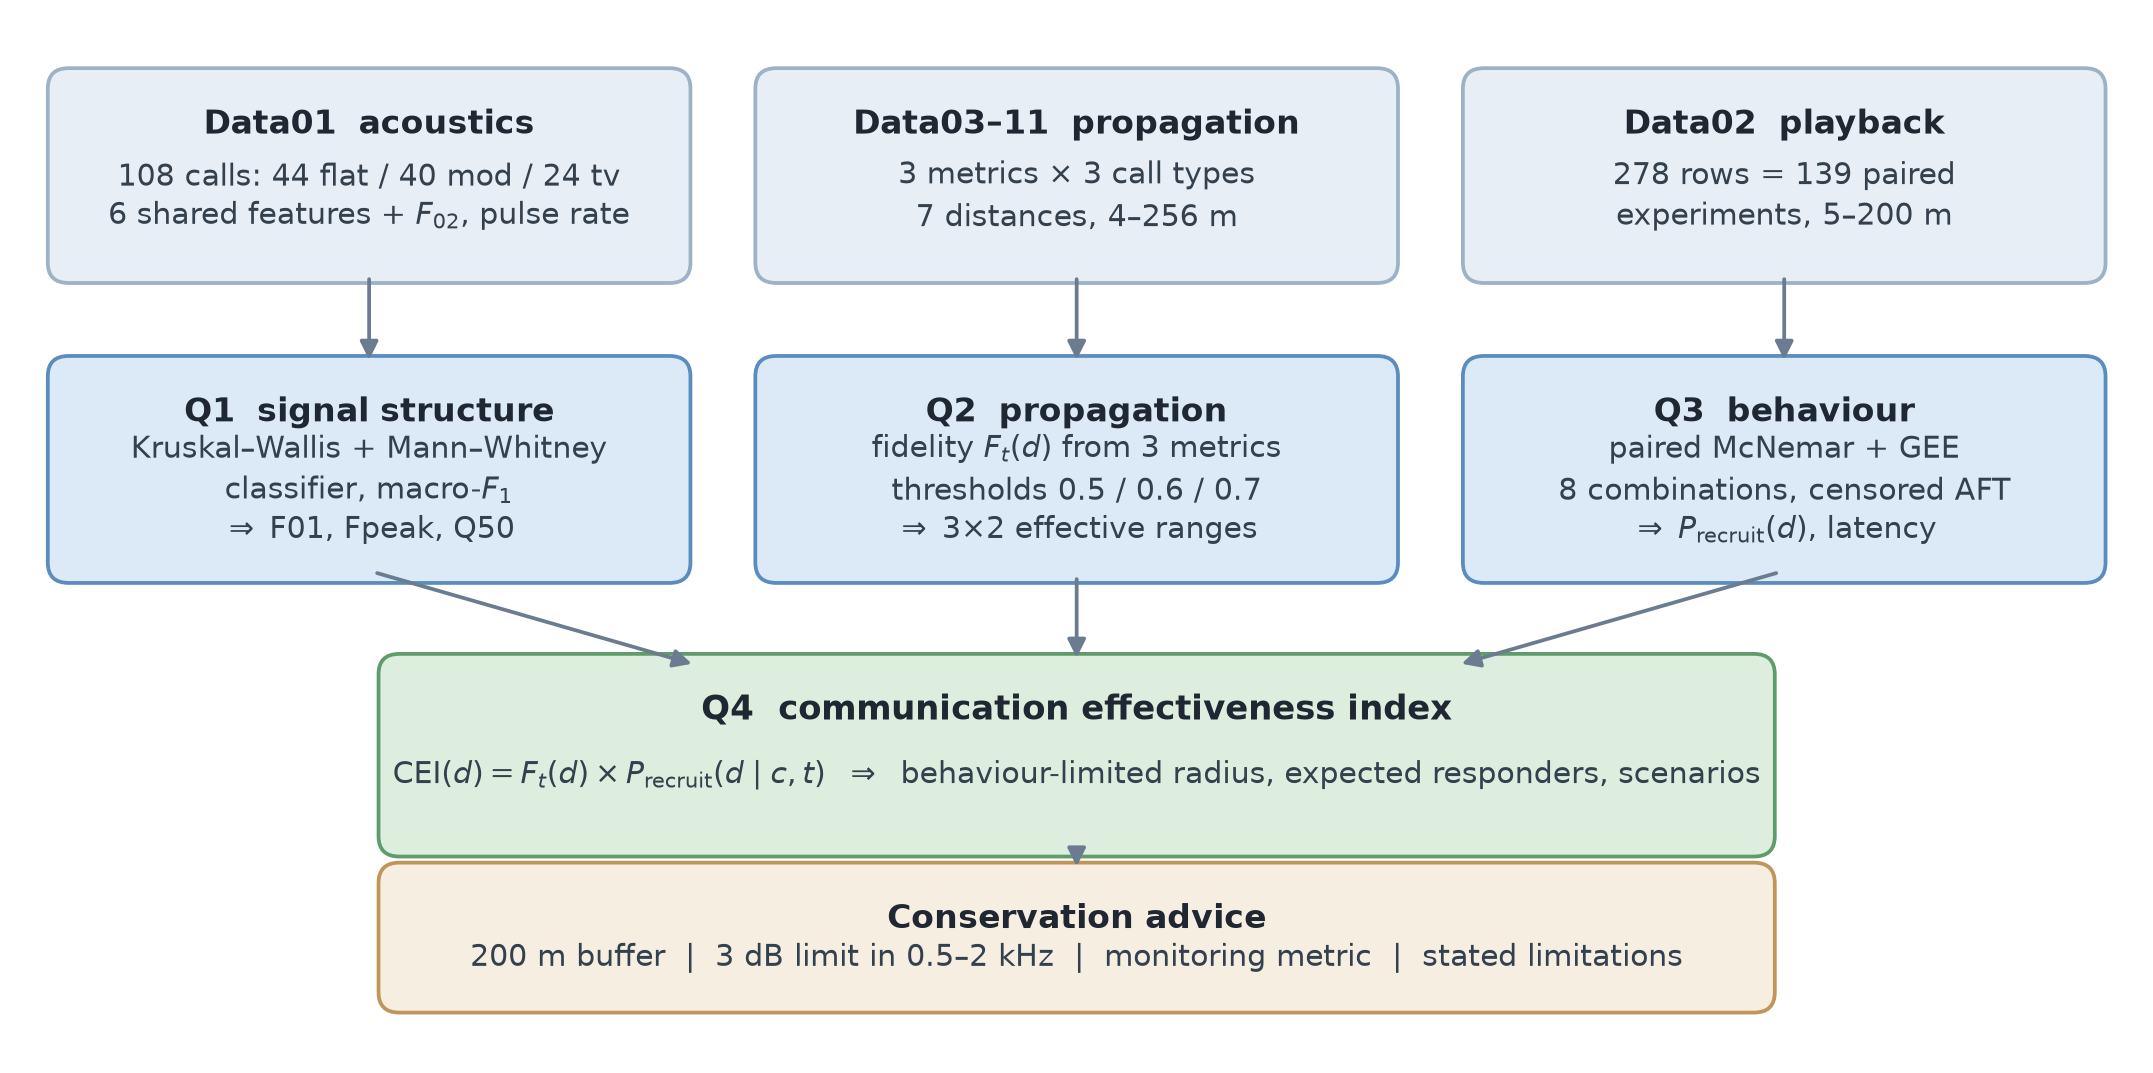
\includegraphics[width=0.80\textwidth]{figs/fig0_route.png}
  \caption{Technical route. Three data sources feed three parallel analyses, which are combined
  into one index and translated into conservation advice.}\label{fig:route}
\end{figure}

The four sections are not four essays; they form one chain, and every link is explicit. Problem~1
returns three spectral indicators (F01, Fpeak, Q50) and the statement that the call types differ
along the frequency axis. Problem~2 returns the fidelity surface $F_t(d)$ built from all three
propagation metrics. Problem~3 returns the recruitment probability
$P_{\mathrm{recruit}}(d\mid c,t)$ and the latency distribution. Problem~4 multiplies the first two
into the index and reads the radii off it. If any link is missing, the next section cannot be
computed: this is why we do not report a single ``combined'' model that would blur the provenance
of each number.

\section{Data, design and notation}\label{sec:data}

\subsection{Three datasets}

The problem supplies three kinds of evidence, summarised in Table~\ref{tab:data}.

\begin{table}[htbp]
  \centering
  \caption{Datasets used in this paper.}\label{tab:data}
  \small
  \begin{tabular}{llll}
    \toprule
    Source & Content & Shape & Used in \\
    \midrule
    Data01 & acoustic measurements of sea-surface calls & 108 calls $\times$ 11 fields & Problem 1 \\
    Data02 & playback trials, paired call/control & 278 rows = 139 pairs $\times$ 40 fields & Problem 3, 4 \\
    Data03--11 & propagation correlations at 7 distances & 9 files $\times$ 300 rows $\times$ 7 distances & Problem 2, 4 \\
    \bottomrule
  \end{tabular}
\end{table}

The acoustic file contains 44 flat, 40 modulated and 24 two-voice calls. Two fields are
\emph{structurally} missing rather than lost: the second fundamental $F_{02}$ exists only for
two-voice calls (24/24 present, 0/84 elsewhere), and the pulse rate is present for modulated
(34/40) and two-voice (20/24) calls but never for flat calls (0/44). This structure is a
property of the call types, and treating it as an ordinary covariate would leak the label into
the classifier; Section~\ref{sec:q1} quantifies that leakage.

\subsection{The paired playback design}\label{sec:paired}

Each of the 139 experiments (\texttt{expID}) contains exactly two rows: one natural call and one
control, played on the same date and in the same behavioural context. This is a matched-pair
design, and it is the single most important structural fact in the dataset. Three consequences
follow.

First, the comparison of interest is within-pair. A test that pools the 139 call rows and the
139 control rows discards the matching and attenuates the effect: the pooled odds ratio is 12.4,
whereas the paired McNemar odds ratio is 37.0 (Section~\ref{sec:q3-overall}).

Second, matching is complete at the level of date and context but not at the level of distance.
All 139 pairs share a date and a context; only 49 pairs share a distance, and the remaining 90
differ by between $-150$ and $+120$ m. Pairing is therefore a group-level device, not a
distance-matched one. We use the pair as the clustering unit (generalised estimating equations
with an exchangeable working correlation) and report an equal-distance subset as a sensitivity
analysis rather than as the primary estimate.

Third, the 139 call trials reuse 28 distinct playback tracks (plus one pseudo-track for the
control), with a mean of 4.96 trials per track. Trials are therefore not independent at the level
of the stimulus either. The track-level intraclass correlation of response is 0.079, which is
small but non-zero; we treat it as a sensitivity dimension rather than as a second random effect
in the primary model, because the number of tracks per call type is small (11, 7 and 10).

\subsection{Derived outcomes and definitional sensitivity}\label{sec:derived}

The response indicators in Data02 are derived quantities, not independent observations. The
identities hold for all 278 rows without exception:
\begin{align}
  \text{HeadsUpYesNo} &= \mathbf{1}\{\text{HeadsUpDuration}>0\}, \\
  \text{ApproachYesNo} &= \mathbf{1}\{\text{ApproachDuration}>0\}, \\
  \text{VocalYesNo} &= \mathbf{1}\{\text{VocalNcalls}>\text{VocalNcallsBefore}\}, \\
  \text{ResponseYesNo} &= \text{HeadsUp} \lor \text{Vocal} \lor \text{Approach}.
\end{align}

The third identity deserves emphasis. \texttt{VocalYesNo} measures a \emph{net increase} over the
pre-playback baseline, not the occurrence of any vocalisation. Four rows therefore have
\texttt{VocalYesNo}$=0$ while \texttt{VocalNcalls}$>0$: the bird vocalised after playback, but
less than it had before. These rows are not data errors, and we do not delete them. To show that
the conclusions do not depend on this convention, we recompute the response counts under three
alternative definitions (Table~\ref{tab:defsens}).

\begin{table}[htbp]
  \centering
  \caption{Definitional sensitivity of the response counts (all 278 rows, calls and controls
  combined). S0 is the primary definition.}\label{tab:defsens}
  \small
  \begin{tabular}{llrrr}
    \toprule
    Scenario & Definition & Vocal events & Any response (278 rows) & of which control \\
    \midrule
    S0 & net increase (primary) & 81 & 108 & 18 \\
    S1 & any post-playback vocalisation & 85 & 111 & 20 \\
    S2 & approach attempt (latency recorded) & 81 & 109 & 18 \\
    S3 & S1 and S2 combined & 85 & 112 & 20 \\
    \bottomrule
  \end{tabular}
\end{table}

Across the three alternatives the total number of any-response trials (calls and controls
combined) moves between 108 and 112, of which 18--20 are controls, so the qualitative conclusions
of Section~\ref{sec:q3} are not an artefact of the definition.

\subsection{The nested structure of the propagation data}

Each of the nine propagation files contains 300 rows and seven columns, one per distance. The
rows are not 300 independent trials. They form 30 contiguous blocks of ten rows, and each block
corresponds to one call-level unit measured at all seven distances. A block indicator alone
explains 55.7\% (two-voice), 72.2\% (flat) and 80.2\% (modulated) of the row-level variance in
fidelity; the median design effect is 6.46, which corresponds to an effective sample size of
about 46 per distance rather than 300. Any interval computed by resampling rows independently is
too narrow by a factor of about 2.5. All uncertainty statements about the CEI radii in
Section~\ref{sec:q4} therefore use a \emph{block} bootstrap that resamples the 30 blocks, not
the rows \cite{ref7}. The Q2 threshold radii in Table~\ref{tab:q2-ranges} use a record-level bootstrap and
should be read as lower bounds; the model-family range is the honest summary.

Within a call type, the missing-value pattern is identical across the three metrics, which
confirms that the three columns describe the same trials and can be averaged row-wise. Across
call types the rows cannot be matched, because no trial identifier is shared; we never assume that
row $i$ of the flat file and row $i$ of the modulated file are the same event.

\subsection{Assumptions}

Four assumptions carry the analysis, and each is stated with the evidence that supports it.

\begin{description}[leftmargin=1.2em,itemsep=2pt]
  \item[A1] \textbf{The three correlations measure one latent fidelity.} Supported by the strong
  correlation between the spectrogram and amplitude-spectrum metrics ($r=0.81$--$0.97$ per call
  type). We nevertheless treat the equal weighting as a choice, not a fact, and vary it in
  Section~\ref{sec:q4-sens}.
  \item[A2] \textbf{The playback pair is exchangeable within an experiment.} Justified by design
  (same date, context and, in 49 pairs, same distance); relaxed by the equal-distance subset.
  \item[A3] \textbf{Censoring is non-informative at $W=60$ s.} The observation window is not
  recorded in the data; 60 s is the upper bound of the duration field and exceeds the largest
  observed latency (47.8 s). We vary $W$ over 48, 90 and 120 s.
  \item[A4] \textbf{Fidelity and recruitment are multiplicatively separable.} This is a modelling
  choice with an ecological justification (two necessary conditions), not a testable law; we say
  so explicitly in Section~\ref{sec:q4}.
\end{description}

\section{Problem 1: acoustic characterisation and classification}\label{sec:q1}

\subsection{What the calls look like}

The dataset contains 108 calls: 44 flat, 40 modulated and 24 two-voice. Six descriptors are
available for every call --- duration, the first fundamental $F_{01}$, the peak frequency, and
the three spectral quartiles --- while two further descriptors exist only for some types. The
second fundamental $F_{02}$ is present for all 24 two-voice calls and for none of the other 84;
the pulse rate is present for 34 of 40 modulated and 20 of 24 two-voice calls but for no flat
call. These are structural properties of the call types, not measurement failures.

Table~\ref{tab:q1-desc} gives the median and interquartile range of the six shared descriptors,
and Figure~\ref{fig:q1-features} shows the full distributions.

\begin{table}[htbp]
  \centering
  \caption{Descriptive statistics of the six shared acoustic features. Median [Q1, Q3].}\label{tab:q1-desc}
  \small
  \begin{tabular}{lrrr}
    \toprule
    Feature & flat ($n=44$) & mod ($n=40$) & tv ($n=24$) \\
    \midrule
    Duration (s) & 0.367 [0.315, 0.432] & 0.394 [0.349, 0.446] & 0.383 [0.344, 0.462] \\
    $F_{01}$ (Hz) & 298.0 [266.8, 310.0] & 287.0 [271.5, 298.5] & 274.5 [263.8, 282.0] \\
    Fpeak (Hz) & 916.0 [825.5, 964.3] & 831.0 [285.0, 906.8] & 829.5 [296.0, 912.8] \\
    Q25 (Hz) & 537.5 [468.0, 622.3] & 501.0 [460.3, 557.3] & 495.0 [407.0, 587.3] \\
    Q50 (Hz) & 908.0 [825.5, 937.0] & 864.5 [821.5, 900.0] & 844.5 [826.8, 891.5] \\
    Q75 (Hz) & 1099.0 [986.0, 1195.8] & 1097.5 [1030.3, 1151.0] & 1083.0 [1018.3, 1118.8] \\
    \midrule
    $F_{02}$ (Hz) & absent & absent & 303.5 [299.8, 315.8] \\
    PulseRate (Hz) & absent & 28.4 [21.7, 35.7] & 31.1 [27.5, 35.3] \\
    \bottomrule
  \end{tabular}
\end{table}

\begin{figure}[htbp]
  \centering
  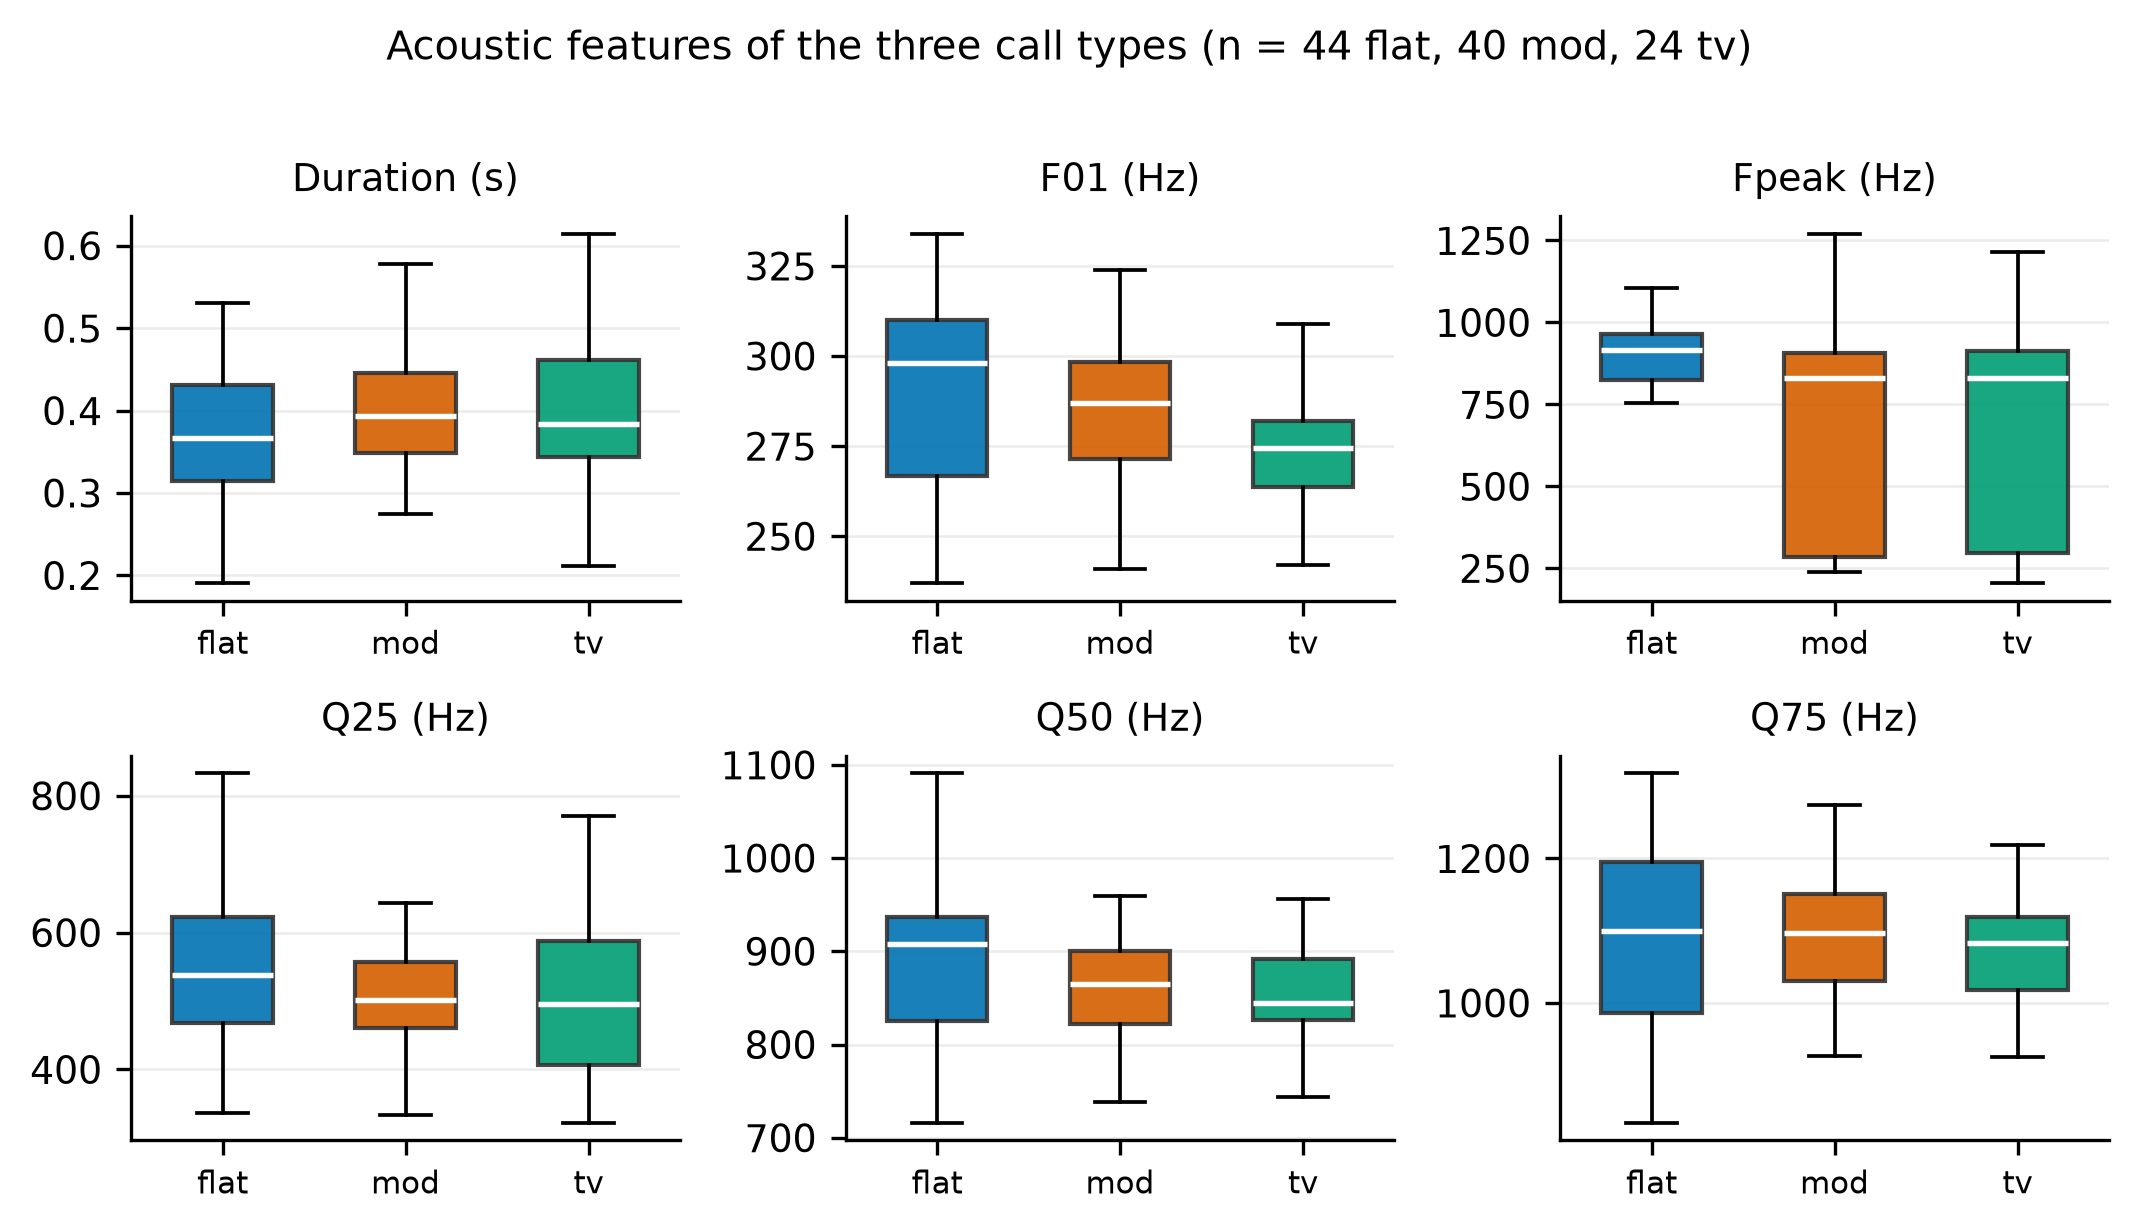
\includegraphics[width=0.78\textwidth]{figs/fig1_features.png}
  \caption{Distributions of the six shared acoustic features by call type. Boxes show the
  interquartile range, the white line the median, and whiskers extend to 1.5 times the
  interquartile range.}\label{fig:q1-features}
\end{figure}

Two features of the table deserve comment before any test is run. First, duration is almost
constant across types (medians 0.367, 0.394 and 0.383 s), so it cannot carry much discriminative
information. Second, the peak frequency has a strongly skewed distribution for modulated and
two-voice calls: the medians are 831 and 830 Hz, but the lower quartiles fall to about 290 Hz
and the means (667 and 676 Hz) sit far below the medians. A handful of low-frequency outliers
therefore inflates the variance, which is why the rank-based tests below are preferable to any
analysis of means.

\subsection{Two nonparametric tests}

We first apply a Kruskal--Wallis test to each of the six shared features and correct the six
$p$-values with the Holm procedure. Only the features that survive this omnibus correction are
then examined pairwise with Mann--Whitney $U$ tests, which are themselves Holm-corrected together
with the modulated--two-voice comparison of pulse rate. Table~\ref{tab:q1-kw} gives the omnibus
results.

\begin{table}[htbp]
  \centering
  \caption{Kruskal--Wallis tests across the three call types, Holm-corrected over six features.}\label{tab:q1-kw}
  \small
  \begin{tabular}{lrrr}
    \toprule
    Feature & $H$ (2 df) & Holm-adjusted $p$ & $\varepsilon^2$ \\
    \midrule
    Duration & 2.523 & 0.850 & 0.005 \\
    $F_{01}$ & 9.144 & 0.052 & 0.068 \\
    Fpeak & 12.280 & 0.013 & 0.098 \\
    Q25 & 2.157 & 0.850 & 0.001 \\
    Q50 & 6.425 & 0.161 & 0.042 \\
    Q75 & 0.520 & 0.850 & 0.000 \\
    \bottomrule
  \end{tabular}
\end{table}

Only peak frequency survives correction. The first fundamental is marginal ($p=0.052$) and the
median frequency does not survive ($p=0.161$), even though both show a monotone decrease from
flat to modulated to two-voice. The effect sizes tell the same story: $\varepsilon^2=0.098$ for
peak frequency against 0.068 for $F_{01}$ and 0.042 for Q50, and essentially zero for duration,
Q25 and Q75.

\begin{table}[htbp]
  \centering
  \caption{Pairwise Mann--Whitney tests for the features examined, Holm-corrected. Rank-biserial
  $r$ is positive when the first type tends to take larger values.}\label{tab:q1-pair}
  \small
  \begin{tabular}{llrr}
    \toprule
    Feature & Comparison & Adjusted $p$ & Rank-biserial $r$ \\
    \midrule
    Fpeak & flat vs mod & 0.0051 & 0.409 \\
    Fpeak & flat vs tv & 0.0314 & 0.379 \\
    Fpeak & mod vs tv & 0.956 & $-0.009$ \\
    PulseRate & mod vs tv & 0.557 & $-0.179$ \\
    \bottomrule
  \end{tabular}
\end{table}

The pairwise tests confirm where the separation lies, and the pattern is not the one a casual
reading of the medians would suggest. Flat
calls differ from both modulated and two-voice calls in peak frequency, but modulated and
two-voice calls do not differ from each other. The difference between call types is therefore
carried mainly by the position of the spectral peak, and only secondarily by $F_{01}$; once flat
is separated, the remaining two types are acoustically close on all continuous descriptors.

\subsection{Classification and the leakage trap}

The problem asks for a classifier and for the macro-averaged $F_1$, not accuracy alone, because
the classes are unbalanced (44/40/24 against a majority-class baseline of 0.407). We fit a random
forest and a multinomial logistic regression under two feature scopes. The \emph{shared} scope
uses the six features available for all calls; the \emph{full} scope adds the presence indicators
for $F_{02}$ and for the pulse rate, together with their missing-value flags. Both are evaluated
with stratified five-fold cross-validation repeated five times, with hyper-parameters tuned by an
inner three-fold split, and additionally by holding out whole recording dates.

\begin{table}[htbp]
  \centering
  \caption{Classification performance (mean over five repeats of stratified five-fold
  cross-validation).}\label{tab:q1-cv}
  \small
  \begin{tabular}{llrrrrr}
    \toprule
    Scope & Model & Accuracy & Macro-$F_1$ & Recall flat & Recall mod & Recall tv \\
    \midrule
    Shared & Random forest & 0.470 & 0.458 & 0.523 & 0.450 & 0.408 \\
    Shared & Logistic & 0.385 & 0.373 & 0.482 & 0.265 & 0.408 \\
    Full & Random forest & 0.944 & 0.952 & 1.000 & 0.850 & 1.000 \\
    Full & Logistic & 0.939 & 0.947 & 0.986 & 0.850 & 1.000 \\
    \midrule
    \multicolumn{2}{l}{Date holdout, shared forest} & 0.389 & 0.363 & --- & --- & --- \\
    \multicolumn{2}{l}{Date holdout, full forest} & 0.944 & 0.952 & --- & --- & --- \\
    \bottomrule
  \end{tabular}
\end{table}

The gap between the two scopes is the most important result in this section, and it is a warning
rather than a success. The full-scope classifier reaches a macro-$F_1$ of 0.952 because the
presence of a second fundamental identifies two-voice calls perfectly and the presence of a pulse
rate identifies flat calls. That is label leakage: the ``feature'' is a restatement of the class.
The honest measure of acoustic separability is the shared-scope result, 0.458, which is only
slightly above the majority-class baseline and collapses to 0.363 when whole dates are held out.
We report both, and we do not claim that the call types are acoustically separable on continuous
descriptors alone.

Permutation importance and significance disagree in one place. Importance concentrates on
$F_{01}$ (0.084) and Q50 (0.033), with Fpeak lower (0.019); significance after Holm correction
selects Fpeak alone. The source analysis resolves this by combining the two views and reports
$F_{01}$, Q50 and Fpeak as the key shared indicators, which is the set carried into
Problems~2 and 3. The disagreement is interpretable rather than troubling: importance measures
how much a tree ensemble uses a feature given the others, whereas the rank test measures marginal
separation, and Fpeak separates flat from the other two while being largely redundant with
$F_{01}$ and Q50 once those are available.

\subsection{Information function and transmission robustness}

The three call types are not three labels for the same signal. The acoustic evidence suggests a
division of labour that the later sections test behaviourally.

Flat calls have the highest first fundamental (298 Hz) and the highest peak frequency (916 Hz),
the narrowest spectral spread, and no pulse structure. A pure tone of this kind is easy to
localise and easy to detect against low-frequency noise, but it carries little fine structure, so
it can signal presence more easily than identity.

Modulated calls add a pulse rate (median 28.4 Hz) and a broader peak distribution. The temporal
modulation provides redundancy in the time domain, which is what survives when the spectrum is
distorted by multipath propagation.

Two-voice calls carry a second fundamental at 303.5 Hz in addition to the first at 274.5 Hz. This
is the only structural feature that is unique to a call type, and it is the feature that makes
the full-scope classifier look excellent. Its function is plausibly redundancy across frequency
bands: if one band is masked by noise, the other still carries the pattern.

These interpretations are hypotheses, not results, and we label them as such. What the data
establish is narrower: the three types differ in where their spectral energy sits and in whether
they carry a second band or a pulse train. Whether those differences matter for transmission is
the question of Section~\ref{sec:q2}, and whether they matter for behaviour is the question of
Section~\ref{sec:q3}.

\paragraph{Hand-off to later sections.}
Three indicators are carried forward: $F_{01}$ as the carrier of the fundamental, Fpeak as the
most statistically distinct descriptor, and Q50 as a robust summary of spectral placement. The
structural indicators ($F_{02}$ present, pulse rate present) are carried forward as \emph{call
type definitions}, not as acoustic covariates, precisely because they would leak the label.

\section{Problem 2: propagation, fidelity and effective range}\label{sec:q2}

\subsection{From three correlations to one fidelity index}

For each call type the archive supplies three correlation series measured against the 1 m
reference recording: a spectrogram correlation, an amplitude-spectrum correlation and an
envelope correlation, each at seven distances from 4 to 256 m. The problem requires all three to
enter the analysis jointly, so we define
\begin{equation}\label{eq:fidelity}
  F_t(d) \;=\; \sum_{m\in\{\mathrm{spec},\mathrm{amp},\mathrm{env}\}} w_m\, r_{m,t}(d),
  \qquad \sum_m w_m = 1 ,
\end{equation}
with equal weights as the baseline. The index lies in $[0,1]$ by construction, since each $r$ is
a correlation, and requires no separate normalisation: at 4 m all three call types already sit
between 0.63 and 0.92, so the scale is anchored by the data rather than by an arbitrary constant.

The three components are not independent evidence. The spectrogram and amplitude-spectrum
correlations are highly correlated across call types (per-type correlations of 0.81--0.97),
although at the level of individual trials the agreement is weaker and varies with distance
(from 0.56 at short range to 0.99). A principal-component analysis of
the three gives a first component explaining 73.5--85.2\% of the variance with loadings of about
0.35, 0.35 and 0.30. Equal weighting therefore places two thirds of the weight on what is
effectively one dimension. We keep equal weights as the baseline because it is the least
assumption-laden choice, report the principal-component weights as an alternative, and treat the
envelope weight as the sensitivity parameter that matters most
(Section~\ref{sec:q2-sens}).

Table~\ref{tab:q2-raw} gives the raw means that enter Equation~\eqref{eq:fidelity}, and
Figure~\ref{fig:q2-fidelity} shows the resulting curves.

\begin{table}[htbp]
  \centering
  \caption{Mean correlation with the 1 m reference recording, by distance, call type and metric
  (s = spectrogram, a = amplitude spectrum, e = envelope). Each value is a mean over the available
  trials of that distance; $n$ varies from 190 to 300.}\label{tab:q2-raw}
  \scriptsize
  \setlength{\tabcolsep}{3.4pt}
  \begin{tabular}{lrrrrrrrrr}
    \toprule
    & \multicolumn{3}{c}{flat} & \multicolumn{3}{c}{mod} & \multicolumn{3}{c}{tv} \\
    \cmidrule(lr){2-4}\cmidrule(lr){5-7}\cmidrule(lr){8-10}
    Distance (m) & s & a & e & s & a & e & s & a & e \\
    \midrule
    4 & 0.908 & 0.923 & 0.650 & 0.872 & 0.876 & 0.675 & 0.824 & 0.825 & 0.626 \\
    8 & 0.892 & 0.868 & 0.595 & 0.913 & 0.918 & 0.754 & 0.880 & 0.880 & 0.634 \\
    16 & 0.905 & 0.918 & 0.657 & 0.841 & 0.844 & 0.656 & 0.789 & 0.790 & 0.515 \\
    32 & 0.869 & 0.755 & 0.529 & 0.834 & 0.847 & 0.560 & 0.811 & 0.819 & 0.506 \\
    64 & 0.733 & 0.712 & 0.343 & 0.842 & 0.860 & 0.599 & 0.846 & 0.849 & 0.562 \\
    128 & 0.412 & 0.453 & 0.211 & 0.618 & 0.680 & 0.362 & 0.740 & 0.772 & 0.449 \\
    256 & 0.166 & 0.192 & 0.170 & 0.250 & 0.278 & 0.223 & 0.318 & 0.371 & 0.139 \\
    \bottomrule
  \end{tabular}
\end{table}


\begin{figure}[htbp]
  \centering
  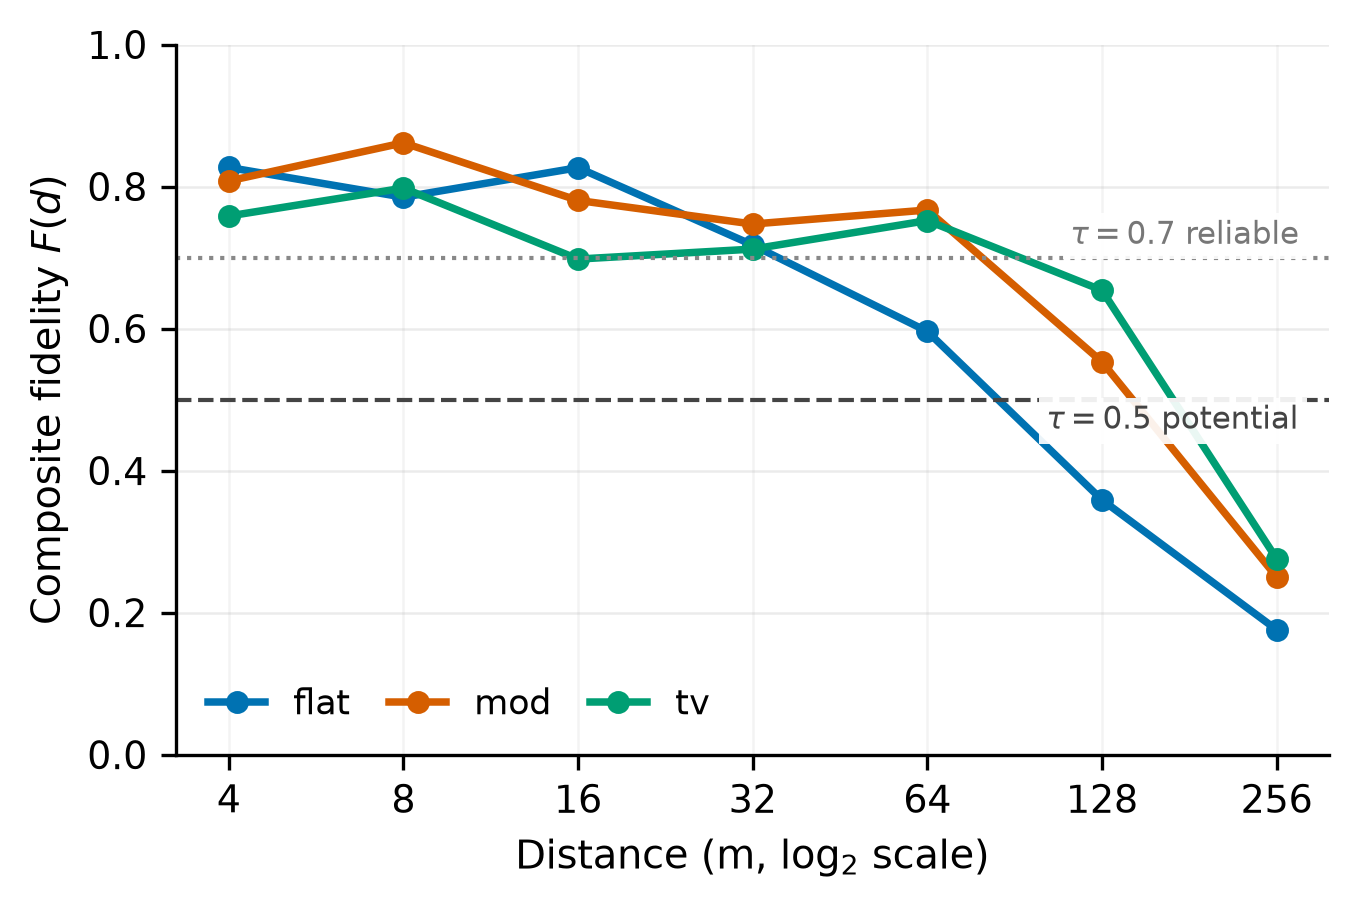
\includegraphics[width=0.44\textwidth]{figs/fig2_fidelity.png}
  \caption{Composite fidelity against distance with the two operational thresholds. The curves
  are not monotone at short range: modulated and two-voice fidelity rise from 4 to 8 m.}\label{fig:q2-fidelity}
\end{figure}

Three patterns are visible before any model is fitted. Fidelity is nearly flat to 32 m for all
three types. It collapses between 64 and 256 m, with the two-voice call retaining the most at
128 m (0.654 against 0.553 for modulated and 0.359 for flat). And the envelope correlation starts
far below the other two (0.65 at 4 m) and contributes the steepest decline, which is why it
behaves as the strictest of the three filters.

\subsection{Three performance models and a threshold scheme}

The problem asks for a separate degradation model for each call type. We fit three families to
the seven distance means, because with seven points the shape of the curve is not identified by
the data alone.

\begin{itemize}[leftmargin=1.5em,itemsep=2pt]
  \item A \textbf{monotone interpolation} on the $\log_2$ distance axis, which imposes only that
        fidelity does not increase with distance. This is the primary curve and the one used for
        the radii reported below.
  \item A \textbf{generalised additive model} $F_t(d)=\beta_0+s_t(d)+\varepsilon$ with a penalised
        spline, mirroring the official analysis code. The effective degrees of freedom are 2.93
        (flat), 2.00 (mod) and 2.88 (tv); the value of exactly 2.00 for modulated means the
        smoother has collapsed to a linear trend, not that the true relation is linear.
  \item Two \textbf{Weibull-type decays}, four-parameter
        $F=b+(a-b)\exp[-(d/\lambda)^k]$ and three-parameter ($b=0$), fitted by constrained
        nonlinear least squares.
\end{itemize}

The threshold scheme converts fidelity into a graded claim about recognisability.
Table~\ref{tab:q2-thresholds} states the three tiers. They are operational definitions chosen to
span the range a receiver might use; the data cannot locate a perceptual boundary, and we do not
claim that they do.

\begin{table}[htbp]
  \centering
  \caption{Three-tier recognition scheme. The two focal criteria are shown in bold.}\label{tab:q2-thresholds}
  \small
  \begin{tabular}{llll}
    \toprule
    Tier & $\tau$ & Reading & Role \\
    \midrule
    Potential recognition & \textbf{0.5} & the signal is still distinguishable from noise & \textbf{focal criterion 1} \\
    Intermediate & 0.6 & the pattern is recoverable with effort & reported for continuity \\
    Reliable recognition & \textbf{0.7} & the pattern is recoverable without effort & \textbf{focal criterion 2} \\
    \bottomrule
  \end{tabular}
\end{table}

\subsection{Effective communication range}

Inverting the monotone curve gives the effective range $d^*(\tau)=\{d: F_t(d)=\tau\}$, computed by
interpolation and reported with a bootstrap interval over the available records.
Table~\ref{tab:q2-ranges} gives the six focal radii together with the intermediate tier.

\begin{table}[htbp]
  \centering
  \caption{Effective range (m) by call type and criterion. Brackets: bootstrap interval over
  records; see the note on interval width in the text.}\label{tab:q2-ranges}
  \small
  \begin{tabular}{lrrr}
    \toprule
    Criterion & flat & mod & tv \\
    \midrule
    Potential, $\tau=0.5$ & 84.7 [83.1, 86.4] & 144.6 [140.6, 148.2] & 169.7 [168.6, 170.9] \\
    Intermediate, $\tau=0.6$ & 62.6 & 109.2 & 141.3 \\
    Reliable, $\tau=0.7$ & 35.4 [32.6, 37.9] & 77.7 [76.1, 79.5] & 79.2 [76.0, 82.5] \\
    \bottomrule
  \end{tabular}
\end{table}

These intervals resample individual records and assume exchangeability, which the data violate:
the 300 rows form 30 blocks of ten, so a block bootstrap would widen them by a factor of about
2.5. The brackets should be read as lower bounds; the model-family range below is the more
honest summary.

At the potential-recognition criterion the ordering is unambiguous: two-voice calls travel
roughly twice as far as flat calls, and the confidence intervals do not overlap. At the
reliable-recognition criterion the two-voice advantage disappears: 79.2 m against 77.7 m for
modulated, with overlapping intervals. This is not a contradiction but a change of question:
a strict criterion asks whether the fine structure survives, and by that standard the two-voice
call is no better than the modulated one.

The long-distance comparison makes the same point quantitatively. A trapezoidal average on the
log-distance axis over 64--256 m gives 0.576 (tv), 0.528 (mod) and 0.372 (flat). At 128 m the
values are 0.654, 0.553 and 0.359, and at 256 m 0.276, 0.250 and 0.176. Two-voice calls lead at
both of these distances, but modulated calls lead at 64 m (0.757 against 0.721), so the
two-voice advantage is a property of the far field rather than of the whole range; the margin
over modulated shrinks from 0.10 at 128 m to 0.03 at 256 m.

\subsection{Sensitivity: weights, thresholds and model family}\label{sec:q2-sens}

Three dimensions move the answer, and two of them move it more than the sampling error does.

\begin{table}[htbp]
  \centering
  \caption{Effective ranges (m) under four fusion weightings, at the two focal thresholds.}\label{tab:q2-sens}
  \small
  \begin{tabular}{llrrr}
    \toprule
    Threshold & Weighting & flat & mod & tv \\
    \midrule
    $\tau=0.5$ & equal & 84.7 & 144.6 & 169.7 \\
               & spectrogram 0.5 & 90.8 & 148.8 & 175.0 \\
               & amplitude spectrum 0.5 & 91.5 & 153.2 & 178.3 \\
               & envelope 0.5 & 71.3 & 129.8 & 155.9 \\
    \midrule
    $\tau=0.7$ & equal & 35.4 & 77.7 & 79.2 \\
               & spectrogram 0.5 & 43.5 & 82.8 & 99.9 \\
               & amplitude spectrum 0.5 & 38.4 & 85.2 & 106.2 \\
               & envelope 0.5 & 25.5 & 66.8 & \textbf{12.1} \\
    \bottomrule
  \end{tabular}
\end{table}

The envelope row at $\tau=0.7$ is the single most consequential number in Problem~2. Putting half
the weight on the envelope correlation cuts the two-voice radius from 79 m to 12 m and reverses
the ranking, because the two-voice envelope correlation at 256 m is the lowest of the three
(0.139 against 0.170 for flat and 0.223 for modulated), even though its spectrogram correlation
is the highest. The claim ``two-voice calls travel furthest'' is therefore true for the spectral
metrics, false for the envelope, and true of the equal-weight composite — a statement about
metric-dependence that we carry into Section~\ref{sec:q4}.

The third dimension is model family. Table~\ref{tab:q2-models} compares the three fitted
families by leave-one-distance-out RMSE.

\begin{table}[htbp]
  \centering
  \caption{Leave-one-distance-out RMSE by model family. Lower is better.}\label{tab:q2-models}
  \small
  \begin{tabular}{lrrr}
    \toprule
    Model & flat & mod & tv \\
    \midrule
    Distance GAM & 0.1232 & 0.0489 & 0.1215 \\
    Four-parameter Weibull & 0.0327 & 0.0603 & 0.1164 \\
    Three-parameter Weibull & 0.0457 & 0.0563 & 0.1163 \\
    \bottomrule
  \end{tabular}
\end{table}

Converting each fitted model into effective distances gives a different picture at each
tier. At $\tau=0.5$ the GAM returns 88.3, 151.8 and 182.1 m for flat, modulated and
two-voice; the three-parameter Weibull returns 89.7, 151.8 and 188.3 m; the four-parameter
Weibull returns 86.6, 146.0 and 144.9 m. At $\tau=0.7$ the corresponding values are 34.0,
64.3 and 89.2 m (GAM) and 35.9, 76.6 and 101.3 m (three-parameter Weibull).

The four-parameter Weibull puts modulated (146.0 m) marginally ahead of two-voice
(144.9 m), whereas the GAM, the three-parameter Weibull and the monotone interpolation all put
two-voice ahead. The four-parameter fit also drives its shape parameter to the imposed upper
bound ($k=10$) and its asymptotic value to the observed 256 m mean, which is a symptom of
over-parameterisation rather than evidence of a steep cliff. We therefore treat the Weibull
fits as model-family sensitivity, not as a replacement for the primary curve.

\subsection{Hand-off to Problem 4}

Problem~4 needs the fidelity surface on the same distance grid as the playback design. We pass on
$F_t(d)$ at 4, 8, 16, 32, 64, 128 and 256 m from the equal-weight composite, together with two
statements that constrain how it may be used: the values at 4--32 m are nearly flat and ordered
differently at different distances (flat leads at 16 m, modulated at 64 m), so no single ordering
holds at short range; and the two-voice advantage at long range is a property of the spectral
metrics, not of the envelope.

\section{Problem 3: behavioural response to playback}\label{sec:q3}

\subsection{Overall response: the paired comparison}\label{sec:q3-overall}

Table~\ref{tab:q3-rates} reports the response rates for the four outcomes. Natural calls
produce a response in 64.8\% of trials and controls in 12.9\%. The gap is not uniform across
behaviours: it is smallest for heads-up (39.6\% versus 9.4\%) and largest for approach, where
no control trial produced a single approach (16.5\% versus 0\%).

\begin{table}[htbp]
  \centering
  \caption{Response rates by outcome and stimulus (n = 139 per group), with Wilson 95\% confidence intervals.}\label{tab:q3-rates}
  \small
  \begin{tabular}{lrrrr}
    \toprule
    Outcome & Call $n$ (\%) & 95\% CI & Control $n$ (\%) & 95\% CI \\
    \midrule
    Any response & 90 (64.8) & 56.4--72.4 & 18 (12.9) & 8.4--19.5 \\
    Heads-up & 55 (39.6) & 31.8--47.9 & 13 (9.4) & 5.6--15.4 \\
    Vocalisation & 76 (54.7) & 46.4--62.8 & 5 (3.6) & 1.6--8.2 \\
    Approach & 23 (16.5) & 11.3--23.6 & 0 (0.0) & 0.0--2.7 \\
    \bottomrule
  \end{tabular}
\end{table}

Because the design is paired, the correct test compares the discordant pairs \cite{ref5}. Table~\ref{tab:q3-pair}
gives the McNemar counts. For any response, 74 pairs favour the call and 2 favour the control,
giving an odds ratio of 37.0 with an exact 95\% confidence interval of 9.9 to 311.

\begin{table}[htbp]
  \centering
  \caption{Paired McNemar tests. $b$: call responds, control does not; $c$: the reverse.}\label{tab:q3-pair}
  \small
  \begin{tabular}{lrrrrr}
    \toprule
    Outcome & $b$ & $c$ & OR & 95\% CI & Exact $p$ \\
    \midrule
    Any response & 74 & 2 & 37.0 & 9.9--311 & $<0.001$ \\
    Heads-up & 45 & 3 & 15.0 & 4.8--75.5 & $<0.001$ \\
    Vocalisation & 73 & 2 & 36.5 & 9.7--307 & $<0.001$ \\
    Approach & 23 & 0 & $\infty$ & $\geq 5.7$ & $<0.001$ \\
    \bottomrule
  \end{tabular}
\end{table}

Two robustness checks qualify this result. First, only 49 of the 139 pairs share a distance.
Restricting to those pairs lowers the odds ratio to 13.5 ($p<0.001$), which is still large but
shows that part of the apparent effect in the full sample comes from the call trials having
been played, on average, slightly closer. We report 37.0 as the design-based estimate and 13.5
as the distance-matched one; both appear in the abstract of the analysis and neither changes
the conclusion. Second, the pooled (unpaired) odds ratio is 12.4 --- close to the matched
subset (13.5) but for the wrong reason, since it ignores the matching entirely. We use the
pooled value nowhere except as an illustration of how much the design matters
(Figure~\ref{fig:q3-rates} shows the rates that underlie these comparisons).

\begin{figure}[htbp]
  \centering
  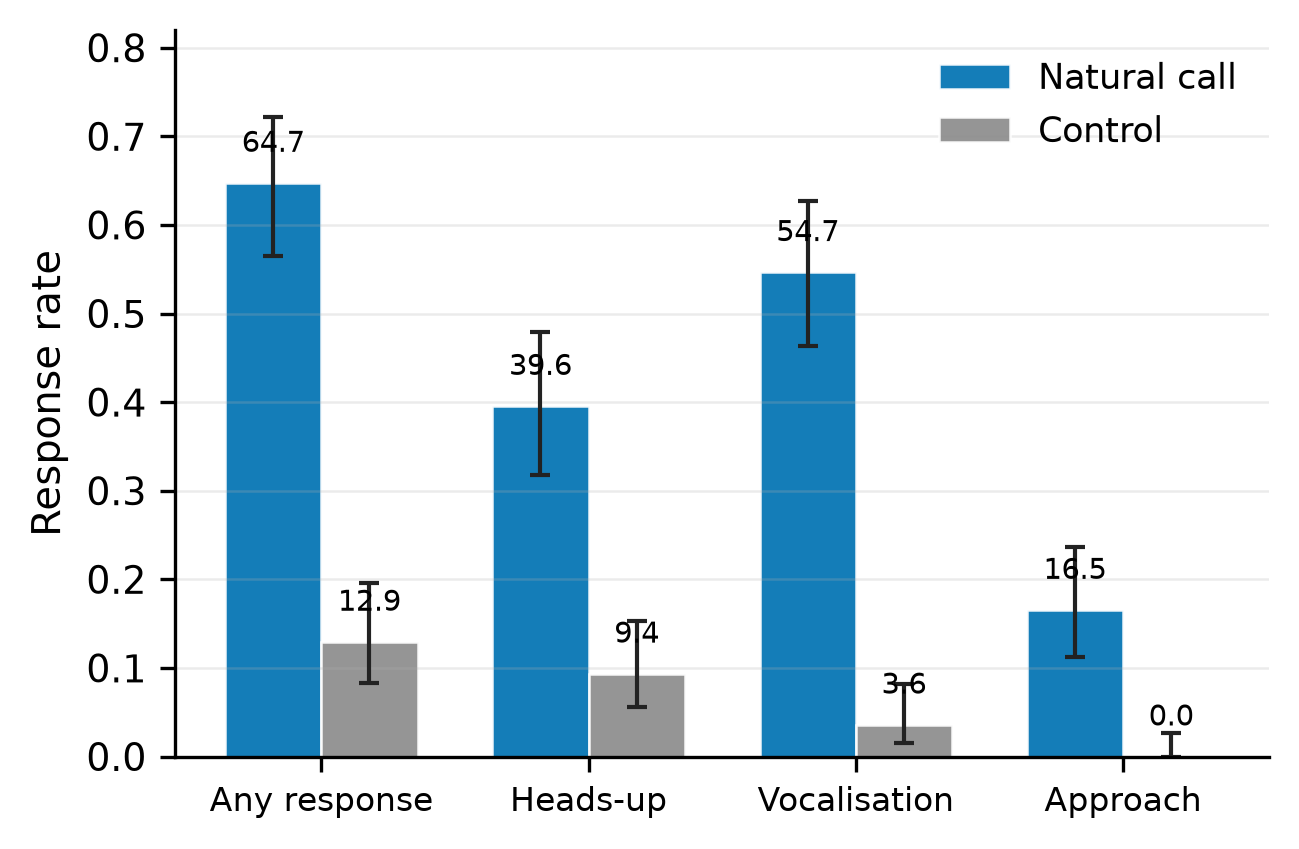
\includegraphics[width=0.40\textwidth]{figs/fig3_rates.png}
  \caption{Response rates by behaviour with Wilson 95\% confidence intervals. The approach
  outcome has no control responses at all.}\label{fig:q3-rates}
\end{figure}

\subsection{Response rates by factor level}\label{sec:q3-strata}

Before fitting a model it is worth seeing the raw structure. Table~\ref{tab:q3-strata}
cross-tabulates response against each factor within the call trials only, so that call and
control are never mixed.

\begin{table}[htbp]
  \centering
  \caption{Response rate by level of each factor, call trials only (n = 139), with Wilson 95\% confidence intervals.}\label{tab:q3-strata}
  \small
  \begin{tabular}{llrrr}
    \toprule
    Factor & Level & $n$ & Responses & Rate \% [95\% CI] \\
    \midrule
    Context & after & 36 & 19 & 52.8 [37.0, 68.0] \\
            & commuting & 65 & 35 & 53.8 [41.9, 65.4] \\
            & searching & 38 & 36 & 94.7 [82.7, 98.5] \\
    \midrule
    Call type & flat & 48 & 29 & 60.4 [46.3, 73.0] \\
              & mod & 33 & 21 & 63.6 [46.6, 77.8] \\
              & tv & 58 & 40 & 69.0 [56.2, 79.4] \\
    \midrule
    Distance & 5--30 m & 13 & 11 & 84.6 [57.8, 95.7] \\
             & 31--60 m & 49 & 31 & 63.3 [49.3, 75.3] \\
             & 61--100 m & 62 & 36 & 58.1 [45.7, 69.5] \\
             & 101--150 m & 10 & 7 & 70.0 [39.7, 89.2] \\
             & 151--200 m & 5 & 5 & 100.0 [56.6, 100.0] \\
    \midrule
    Group size & 1--3 & 39 & 35 & 89.7 [76.4, 95.9] \\
               & 4--8 & 34 & 23 & 67.6 [50.8, 80.9] \\
               & 9--15 & 32 & 21 & 65.6 [48.3, 79.6] \\
               & 16--40 & 34 & 11 & 32.4 [19.1, 49.2] \\
    \bottomrule
  \end{tabular}
\end{table}

Three features of this table drive the modelling choices. The context contrast is dramatic in
the raw data (94.7\% in searching versus about 53\% otherwise) but the searching cell contains
almost only small groups, so it cannot be read as a context effect. Distance is non-monotone:
the 101--150 m and 151--200 m bands have higher rates than the 61--100 m band, but they contain
10 and 5 trials respectively, and the 100\% cell is five trials. Group size is the only factor
with a clean monotone gradient across all four bands. This is why the multivariable model of
Section~\ref{sec:q3-factors} is necessary and why the raw table is not sufficient.

\subsection{Four factors within one framework}\label{sec:q3-factors}

The problem asks for context, call type, distance and group size to be examined in a common
model. We fit a generalised estimating equation \cite{ref4} with a logit link, an exchangeable working
correlation within experiment, and the four factors as additive terms:
\begin{equation}\label{eq:gee}
  \operatorname{logit}\,\Prob(R_{ij}=1)
  = \beta_0 + \beta_{\mathrm{CT}} + \beta_C + \beta_D \log d_{ij} + \beta_N N_{ij},
\end{equation}
where $i$ indexes the experiment and $j$ the row within it. The model uses all 278 rows and
returns population-averaged odds ratios; Table~\ref{tab:q3-gee} gives the estimates and
Figure~\ref{fig:q3-forest} displays them.

\begin{table}[htbp]
  \centering
  \caption{GEE estimates for any response (n = 278, 139 clusters). OR: odds ratio.}\label{tab:q3-gee}
  \small
  \begin{tabular}{lrrr}
    \toprule
    Term & OR & 95\% CI & $p$ \\
    \midrule
    flat vs control & 13.75 & 6.58--28.73 & $<0.001$ \\
    mod vs control & 16.28 & 6.39--41.47 & $<0.001$ \\
    tv vs control & 22.38 & 9.47--52.89 & $<0.001$ \\
    $\log$ distance (per $e$-fold) & 0.491 & 0.291--0.829 & 0.008 \\
    Group size (per bird) & 0.939 & 0.899--0.981 & 0.0045 \\
    Context: commuting vs after & 0.834 & 0.344--2.023 & 0.688 \\
    Context: searching vs after & 1.875 & 0.688--5.111 & 0.219 \\
    \bottomrule
  \end{tabular}
\end{table}

\begin{figure}[htbp]
  \centering
  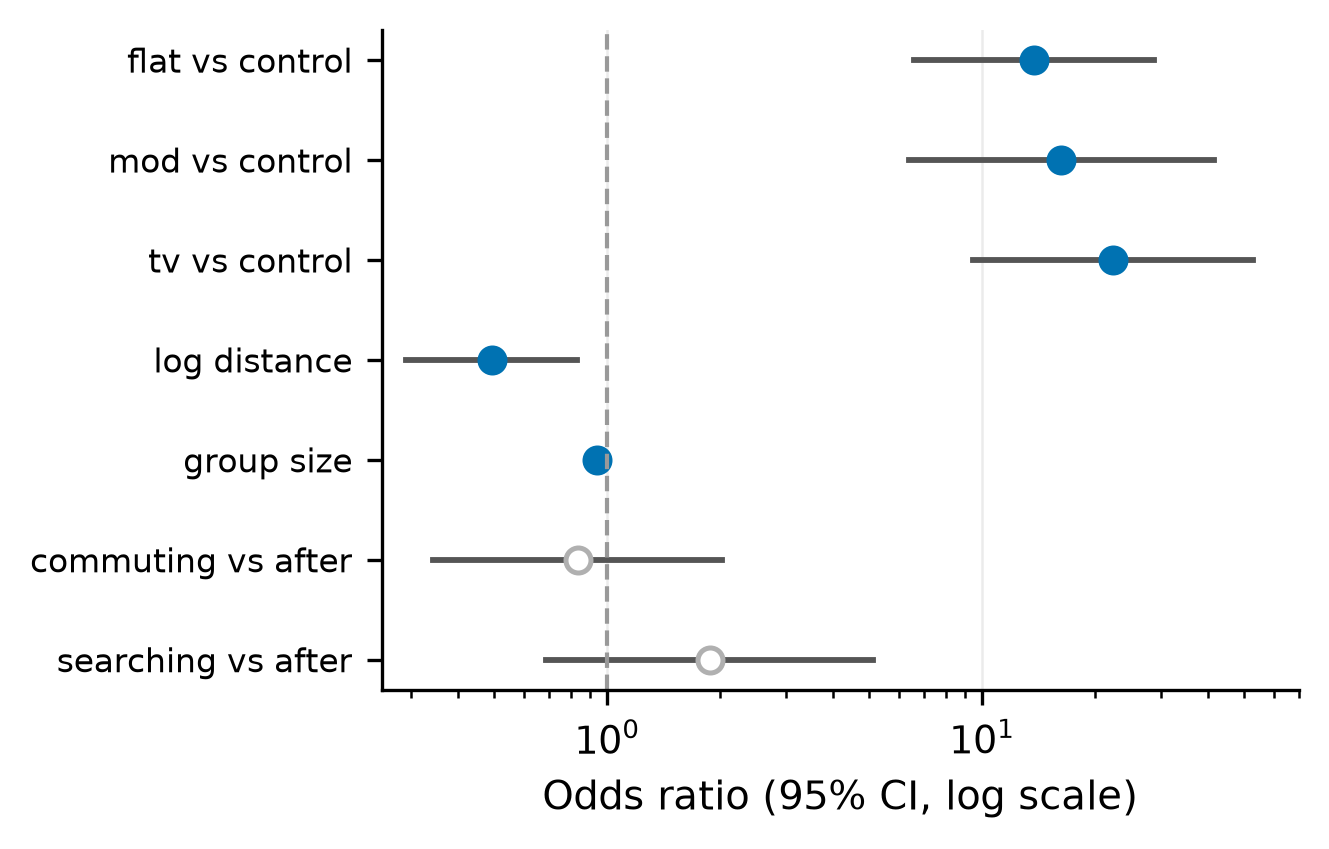
\includegraphics[width=0.40\textwidth]{figs/fig5_forest.png}
  \caption{Adjusted odds ratios from Equation~\eqref{eq:gee}. Filled markers indicate
  $p<0.05$; open markers are not significant.}\label{fig:q3-forest}
\end{figure}

Three readings matter. First, all three call types differ strongly from the control, and the
point estimates increase from flat (13.7) through modulated (16.3) to two-voice (22.4); the
confidence intervals overlap, so this ordering is suggestive rather than established. Second,
response falls with distance: each $e$-fold increase in distance multiplies the odds by 0.49,
so a bird at 140 m has roughly half the odds of responding compared with one at 50 m. Third,
and counter-intuitively, response falls with group size: each additional bird multiplies the
odds by 0.94, so a group of 20 has about half the odds of a group of 8.

Context is not significant after adjustment. This is unsurprising once the confound is seen:
the median group size is 2 in the searching context and 15 in commuting, so the raw contrast
between contexts is largely a contrast between small and large groups. We therefore report the
context coefficients but do not interpret them, and we treat group size as the substantive
variable. This is an association, not a causal effect: large groups may respond less because of
dilution of individual attention, or because an observer is less likely to detect the response
of any particular bird in a large group. The data cannot separate these mechanisms.

\subsection{The eight response combinations}\label{sec:q3-combos}

The three behaviours generate eight combinations. Table~\ref{tab:q3-combos} and
Figure~\ref{fig:q3-combos} show their distribution. The dominant pattern under playback is
vocalisation, alone or combined with heads-up; under control, 87.1\% of trials fall in the
no-response cell and the remaining cells are almost entirely heads-up only.

\begin{table}[htbp]
  \centering
  \caption{Response-combination shares. H = heads-up, V = vocalisation, A = approach.}\label{tab:q3-combos}
  \small
  \begin{tabular}{llrr}
    \toprule
    Code & Combination & Call (\%) & Control (\%) \\
    \midrule
    000 & none & 49 (35.3) & 121 (87.1) \\
    100 & H only & 10 (7.2) & 13 (9.4) \\
    010 & V only & 29 (20.9) & 5 (3.6) \\
    001 & A only & 1 (0.7) & 0 (0.0) \\
    110 & H and V & 28 (20.1) & 0 (0.0) \\
    101 & H and A & 3 (2.2) & 0 (0.0) \\
    011 & V and A & 5 (3.6) & 0 (0.0) \\
    111 & H, V and A & 14 (10.1) & 0 (0.0) \\
    \bottomrule
  \end{tabular}
\end{table}

\begin{figure}[htbp]
  \centering
  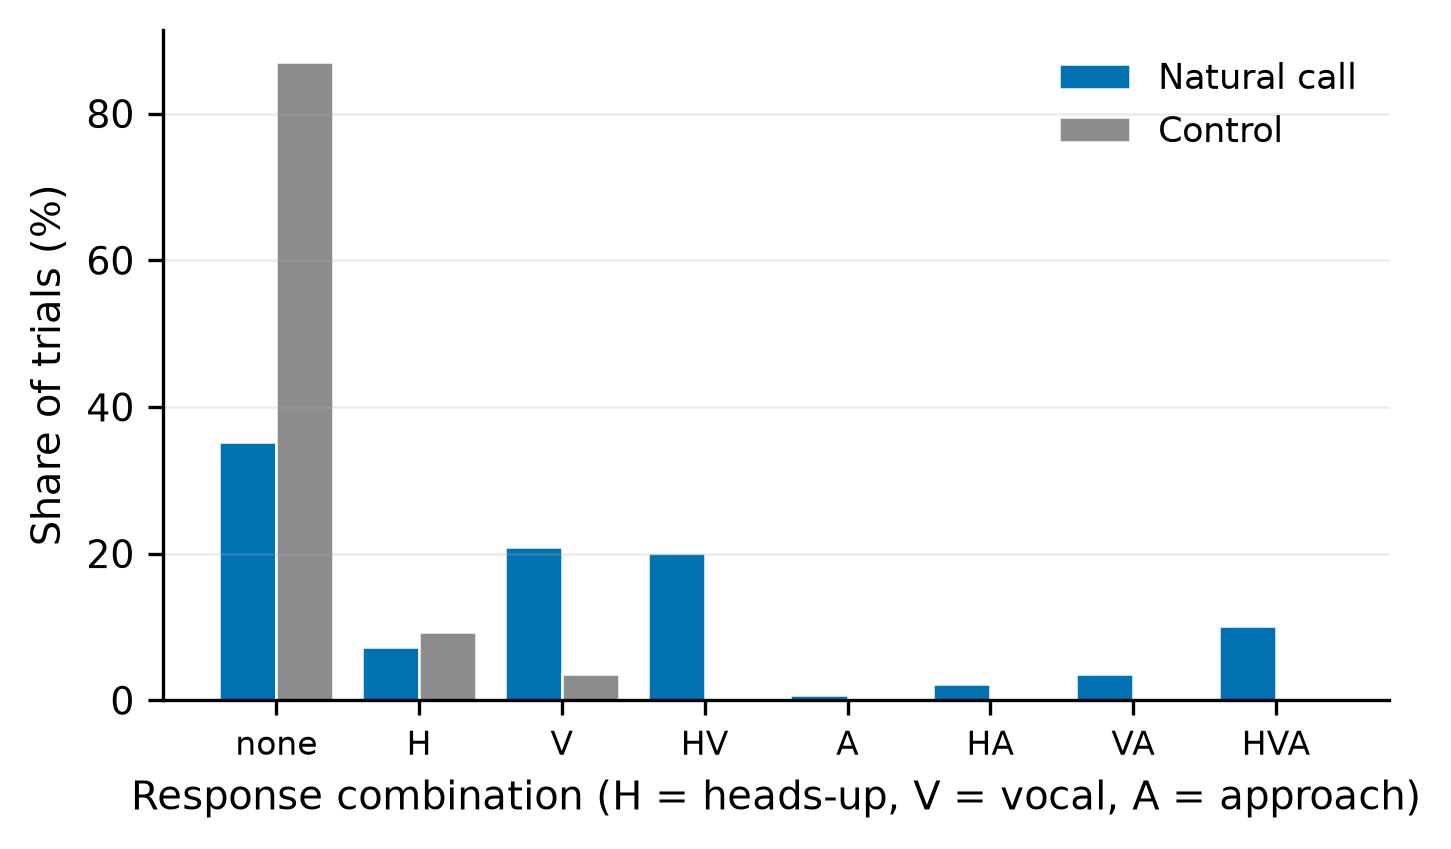
\includegraphics[width=0.42\textwidth]{figs/fig4_combos.png}
  \caption{Share of trials in each response combination.}\label{fig:q3-combos}
\end{figure}

Testing whether playback changes the distribution requires a paired test, because the two
distributions come from the same 139 experiments. A Stuart--Maxwell test \cite{ref6} on the $8\times8$
paired table gives $W=72.9$ on 7 degrees of freedom ($p<0.001$); a permutation test that swaps
call and control labels within each pair 5000 times gives $p=0.0002$. The permutation value is
the more conservative of the two and is the one we quote, because the asymptotic Stuart--Maxwell
statistic is sensitive to the many structurally empty cells.

Whether \emph{call type} shifts the probability of a \emph{specific} combination is a different
question, and here the data are thin. A contingency test of call type by combination among call
trials gives $p=0.137$, with 58\% of expected cell counts below five. We report this as a
directional observation --- two-voice calls produce more approach behaviour and less vocal-only
behaviour than flat calls --- and explicitly as a power limitation, not as evidence of
equivalence.

\subsection{Time to response}\label{sec:q3-latency}

Define the response time as the earliest of the three latencies,
$T=\min(T_H,T_V,T_A)$. A trial in which no behaviour occurs is right-censored at the observation
window $W=60$ s. Of the 108 responding trials (90 call, 18 control), nine have a latency of zero; these are immediate
reactions recorded at the resolution of the observation protocol, and we exclude them from the
latency model while reporting them separately, because a point mass at zero is not compatible
with a continuous log-normal likelihood.

The model is two-part. The first part is the response probability from
Equation~\eqref{eq:gee}. The second part is a log-normal accelerated-failure-time model fitted to
the responders with experiment-level clustering:
\begin{equation}\label{eq:aft}
  \log T_i = \beta_0 + \beta_{\mathrm{CT}} + \beta_C + \beta_D \log d_i + \beta_N N_i
  + \varepsilon_i, \qquad \varepsilon_i \sim N(0,\sigma^2).
\end{equation}
Coefficients are reported as time multipliers, $\exp(\beta)$: a value above one means a longer
time to respond.

\begin{table}[htbp]
  \centering
  \caption{Two-part log-normal AFT model for time to first response among the 99 trials that
  responded and were not immediate (90 call, 18 control, minus nine zero latencies). The reference
  category is control, so each call type is compared with the control stimulus.}\label{tab:q3-aft}
  \small
  \begin{tabular}{lrrr}
    \toprule
    Term & Time multiplier $\exp(\beta)$ & 95\% CI & $p$ \\
    \midrule
    flat vs control & 1.066 & 0.63--1.80 & 0.811 \\
    mod vs control & 0.970 & 0.58--1.63 & 0.909 \\
    tv vs control & 1.354 & 0.76--2.40 & 0.301 \\
    $\log$ distance (per $e$-fold) & 1.265 & 1.08--1.48 & 0.004 \\
    Group size (per bird) & 1.000 & 0.98--1.02 & 0.969 \\
    Context: commuting vs after & 0.810 & 0.56--1.17 & 0.259 \\
    Context: searching vs after & 0.735 & 0.49--1.10 & 0.139 \\
    \midrule
    $\sigma$ (log-scale) & \multicolumn{3}{r}{0.754} \\
    \bottomrule
  \end{tabular}
\end{table}

Only distance matters. Each $e$-fold increase in distance lengthens the expected time to
response by a factor of 1.27 (95\% CI 1.08--1.48, $p=0.004$). No call type differs from the
control stimulus, and the three call-type multipliers lie within 40\% of one another
(0.97--1.35), so call type does not detectably change latency once a bird has decided to respond;
group size does not either. This is consistent with the idea that these factors act on the
decision to respond rather than on the speed of the response.

Two summaries must be reported together, because they answer different questions. The
\emph{conditional} median latency --- the median among birds that respond --- is about 2 s for
heads-up, 3.1 s for vocalisation and 8 s for approach, with an overall first-response median of
2 s (IQR 1--4 s). The \emph{unconditional} restricted mean survival time
$\mathrm{RMST}(60)=\int_0^{60}S(t)\,dt$ \cite{ref8} keeps the non-responders in the denominator and answers
the manager's question: after a single playback, how much response time should be expected on
average? RMST is always the larger of the two numbers and cannot be smaller than the conditional
median multiplied by the response probability.

Figure~\ref{fig:q3-km} shows the Kaplan--Meier curves by call type. The curves separate mainly
in their height rather than their slope: two-voice calls leave fewer birds unanswered at every
time point, but the birds that do answer take slightly longer. This is exactly the pattern that
a single ``mean latency'' would hide, and it is why the conditional median and the RMST are
both reported.

\begin{figure}[htbp]
  \centering
  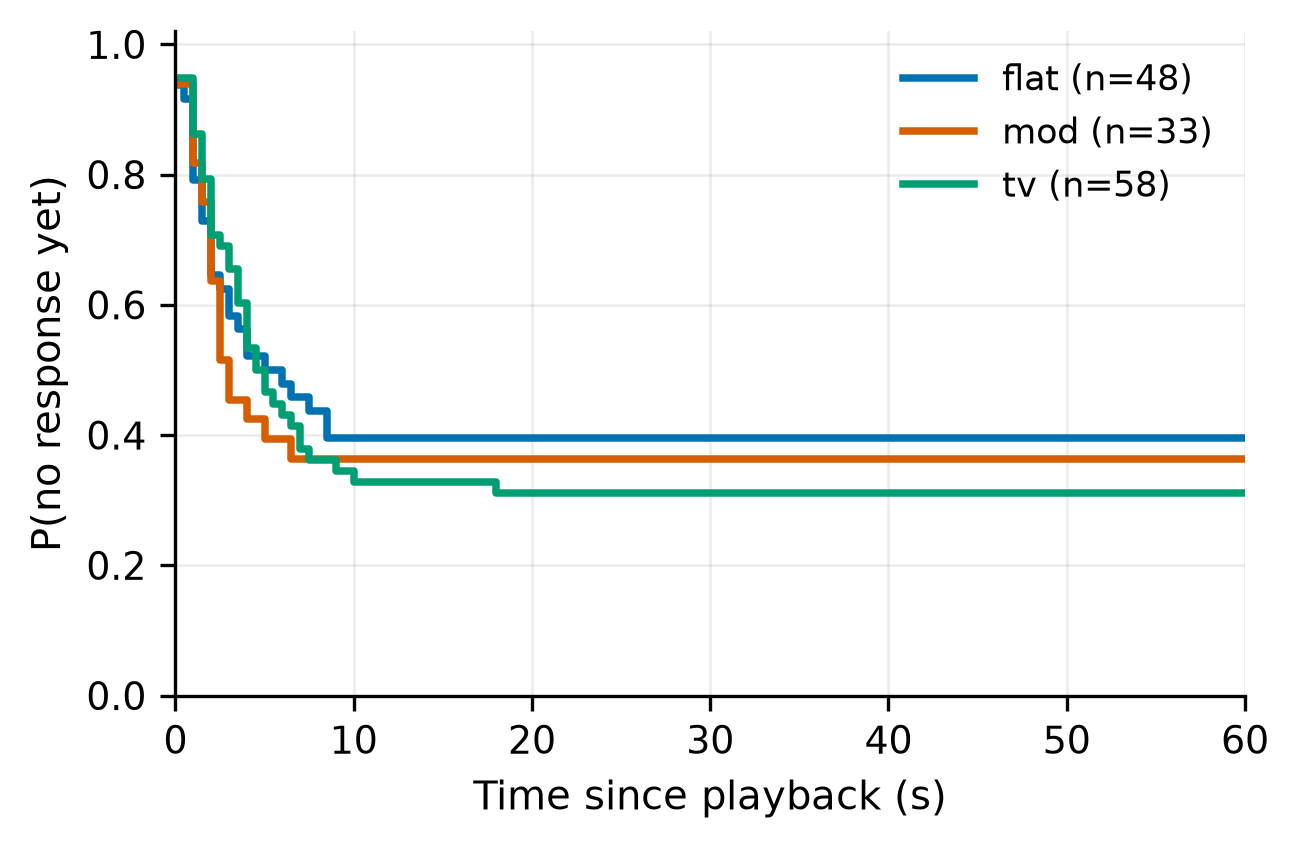
\includegraphics[width=0.40\textwidth]{figs/fig6_km.png}
  \caption{Kaplan--Meier curves of time to first response by call type, with non-responders
  censored at 60 s.}\label{fig:q3-km}
\end{figure}

\subsection{Representative numerical predictions}\label{sec:q3-table}

Table~\ref{tab:q3-pred} gives the required numerical table for a representative group of eight
penguins in the commuting context, at 50, 100 and 150 m. Every cell is a model prediction from
Equations~\eqref{eq:gee} and~\eqref{eq:aft}; none is a raw average. The response probability
falls by 11--12 percentage points from 50 to 100 m and by about 7 points from 100 to 150 m, and the ordering of call
types by response probability (two-voice $>$ modulated $>$ flat) is stable across the three
distances.

\begin{table}[htbp]
  \centering
  \caption{Predicted response probability, conditional median latency and restricted mean
  survival time. Conditions: $N=8$, commuting context.}\label{tab:q3-pred}
  \small
  \begin{tabular}{llrrr}
    \toprule
    Call type & Distance (m) & $P(\text{response})$ & Median latency (s) & $\mathrm{RMST}(60)$ (s) \\
    \midrule
    flat & 50 & 0.638 & 2.16 [1.53, 3.05] & 23.5 \\
    flat & 100 & 0.519 & 2.54 [1.75, 3.70] & 30.6 \\
    flat & 150 & 0.447 & 2.80 [1.87, 4.19] & 34.8 \\
    mod & 50 & 0.676 & 1.97 [1.35, 2.86] & 21.2 \\
    mod & 100 & 0.561 & 2.32 [1.56, 3.43] & 28.1 \\
    mod & 150 & 0.489 & 2.55 [1.67, 3.87] & 32.3 \\
    tv & 50 & 0.742 & 2.75 [2.07, 3.63] & 18.2 \\
    tv & 100 & 0.637 & 3.23 [2.41, 4.34] & 24.5 \\
    tv & 150 & 0.568 & 3.55 [2.58, 4.90] & 28.6 \\
    \bottomrule
  \end{tabular}
\end{table}

The table contains an apparent paradox worth pointing out. Two-voice calls have the highest
response probability at every distance but also the longest conditional median latency. The
reason is that the conditional median is computed among responders, while the response
probability determines how many responders there are. Once both are combined into the RMST,
two-voice calls produce the \emph{smallest} expected waiting time (18.2 s at 50 m versus 23.5 s
for flat), because more birds respond early enough to matter. Reporting only one of the three
columns would reverse the apparent conclusion.

\subsection{No response is not no perception}\label{sec:q3-perception}

The problem states that non-response must be treated as no response but must not be read as
evidence that the stimulus was not perceived. We formalise the distinction by decomposing the
response probability into a perception term and a willingness term:
\begin{align}
  \Prob(\text{response}) &= q(d)\; r(d) ,\label{eq:decomp}\\
  \Prob(\text{not perceived}) &= 1-q(d),\\
  \Prob(\text{perceived but no response}) &= q(d)\bigl(1-r(d)\bigr),
\end{align}
where $q(d)$ is the probability that the call is recognised at distance $d$ and $r(d)$ is the
probability of responding conditional on recognition.

The decomposition is useful but not identifiable from the playback data alone: for any observed
response probability one can trade a lower $q$ against a higher $r$. We therefore take $q$ from
the propagation data, as an external input, and report the result as a framework rather than as
an estimate. Two statements follow.

First, $q(d)=1$ is a hard upper bound on perception. Under that bound, at 100 m the flat call
leaves 48.1\% of trials in the ``perceived but did not respond'' category and no trial in the
``not perceived'' category. Second, the propagation-derived fidelity is \emph{not} a perception
probability: at 100 m the composite fidelity of the flat call is about 0.44, which is below the
observed response probability of 0.52. The two quantities live on different scales, and equating
them would imply a response probability exceeding the perception probability, which is
impossible. We therefore use $F(d)$ only as a monotone index of recognition difficulty and
report $q=1$ as the upper bound, with $q\in[0.5,1]$ as a sensitivity grid.

What the data do support is the qualitative statement, repeated in
Section~\ref{sec:q4}: non-response is a mixture of two mechanisms that the experiment cannot
separate, and any conservation rule that treats silence as absence of perception will
underestimate the distance at which penguins are still affected by noise.

\section{Problem 4: communication effectiveness and conservation}\label{sec:q4}

\subsection{Why a product, not a weighted sum}\label{sec:q4-form}

The problem asks for an index that integrates signal fidelity, response-combination
probabilities and context, with an explicit functional form and an ecological interpretation of
its weights. We define the Communication Effectiveness Index as
\begin{equation}\label{eq:cei}
  \boxed{\;\mathrm{CEI}(d \mid c, t) \;=\; F_t(d)\;\times\;P_{\mathrm{recruit}}(d \mid c, t)\;}
\end{equation}
where $F_t(d)$ is the composite fidelity of call type $t$ at distance $d$ from
Section~\ref{sec:q2}, and $P_{\mathrm{recruit}}(d\mid c,t)$ is the probability that a bird
approaches or vocalises, estimated from the playback model of Section~\ref{sec:q3} for context
$c$.

The multiplicative form is a modelling decision with a biological justification. A weighted sum
$w_1F+w_2P$ allows compensation: a signal that cannot be heard at all ($F=0$) but is played in a
context where birds are eager to respond ($P=1$) would score the same as an audible signal in an
indifferent context. Ecologically these are not equivalent, because the second case still
transmits information while the first transmits nothing. Multiplication encodes two necessary
conditions: if the signal is not audible it cannot recruit, and if the bird is not willing it
will not recruit, regardless of audibility. The cost of this choice is that $F$ and $P$ are
positively correlated, so the index should be read as a structural decomposition rather than as
a causal product. The data also show that the two factors are not equally distance-dependent:
fidelity falls steeply beyond 64 m, whereas the recruitment probability declines only weakly
with distance (OR 0.87 per $e$-fold, 95\% CI 0.53--1.44, $p=0.59$). The radius is therefore
driven mainly by the physics of the signal, and the behavioural term acts as a near-constant
scaling of it.

\subsection{Components and the ecological meaning of the weights}\label{sec:q4-weights}

The fidelity term is itself a weighted average of three correlations,
\begin{equation}\label{eq:fid}
  F_t(d) = w_{\mathrm{spec}} r_{\mathrm{spec},t}(d)
         + w_{\mathrm{amp}}  r_{\mathrm{amp},t}(d)
         + w_{\mathrm{env}}  r_{\mathrm{env},t}(d),
  \qquad \sum_m w_m = 1 .
\end{equation}

Each component measures a different kind of redundancy, and the weights are therefore
interpreted as hypotheses about which kind of redundancy carries recognition.

\begin{table}[htbp]
  \centering
  \caption{Components of the index and their ecological interpretation.}\label{tab:q4-weights}
  \small
  \begin{tabular}{llll}
    \toprule
    Component & What it preserves & Ecological reading & Weight \\
    \midrule
    $r_{\mathrm{spec}}$ & time--frequency structure & identity of the caller & 1/3 (0.35 under PCA) \\
    $r_{\mathrm{amp}}$ & spectral envelope & timbre and body size & 1/3 (0.35 under PCA) \\
    $r_{\mathrm{env}}$ & temporal fluctuation & rhythm and pulse pattern & 1/3 (0.30 under PCA) \\
    $P_{\mathrm{recruit}}$ & approach or vocalisation & willingness to join & multiplier, not a weight \\
    \bottomrule
  \end{tabular}
\end{table}

The equal weights are the neutral choice, but they are not innocent: the spectrogram and
amplitude-spectrum correlations are strongly correlated across call types ($r=0.81$--$0.97$), so equal
weighting places two thirds of the weight on what is effectively one dimension. The first
principal component of the three correlations gives normalised weights close to equal (about
0.37, 0.35 and 0.29 in our recomputation), so an equal-weight and a principal-component composite
produce similar fidelity curves. We keep equal weights as the baseline because they require fewer
assumptions, and report the principal-component alternative in the sensitivity analysis. The envelope correlation is the only component that is substantially
independent of the other two, and it is also the component that starts lowest (0.65 at 4 m) and
collapses fastest. It therefore acts as the strictest of the three filters, which is why it
deserves weight even though it is small in magnitude.

Context enters through $P_{\mathrm{recruit}}$, because the playback model already conditions on
context. Multiplying by a separate context factor would count it twice; we do not do so.

\subsection{Effective communication radius}\label{sec:q4-radius}

Two calibration rules are defensible, and we report both.

\begin{itemize}[leftmargin=1.6em,itemsep=3pt]
  \item \textbf{Behaviour-limited (primary).} $\kappa = 0.5\,\mathrm{CEI}(50\,\mathrm{m})$, held
        fixed at its baseline value in every scenario, that is,
        the distance at which communication effectiveness has fallen to half of its value at a
        distance where every call type is still fully audible. This rule adapts to the absolute
        level of the index and is the one we use for management advice.
  \item \textbf{Signal-limited (reference).} $F(d)=\tau$, that is, the distance at which the signal
        itself falls below a recognition threshold. This quantity ignores behaviour and is
        reported only for comparison; it is not the quantity the problem asks for.
\end{itemize}

\begin{table}[htbp]
  \centering
  \caption{Effective radii (m). Behaviour-limited radii use $\kappa=0.5\,\mathrm{CEI}(50\,\mathrm{m})$;
  signal-limited radii use $F(d)=0.5$. Brackets: block-bootstrap 95\% interval.}\label{tab:q4-radius}
  \small
  \begin{tabular}{lrrr}
    \toprule
    Criterion & flat & mod & tv \\
    \midrule
    Behaviour-limited, empirical curve & 136.6 [131.4, 143.0] & 174.8 [167.3, 181.1] & 203.4 [198.2, 209.2] \\
    Behaviour-limited, logistic fit & 135.7 & 175.9 & 157.8 \\
    Absolute $\mathrm{CEI}=0.20$, empirical & 115.7 [112.3, 118.7] & 158.7 [149.5, 167.5] & 215.6 [211.0, 220.6] \\
    Signal-limited $F=0.5$ & 84.7 [83.1, 86.4] & 144.6 [140.6, 148.2] & 169.7 [168.6, 170.9] \\
    \bottomrule
  \end{tabular}
\end{table}

The behaviour-limited radius is larger than the signal-limited one for every call type, which is
expected: a bird can respond to a partially degraded signal, so the behavioural boundary lies
beyond the physical one. The gap is largest for flat calls (137 versus 85 m) and smallest for
two-voice calls (203 versus 170 m).

The model-family comparison matters more than the confidence intervals. For two-voice calls the
empirical curve gives 203 m but a logistic fit gives 158 m, a difference of 45 m that dwarfs the
bootstrap interval of $\pm5$ m. The reason is visible in Figure~\ref{fig:q2-fidelity}: the raw
mean fidelity of the two-voice call is non-monotone (it rises from 8 to 64 m), so a monotone
parametric curve must cut through the plateau and cross the threshold earlier. We therefore quote
the two-voice radius as a \emph{range} of 158--203 m rather than as a point estimate.
Figure~\ref{fig:q4-cei} shows the index itself with bootstrap bands.

\begin{figure}[htbp]
  \centering
  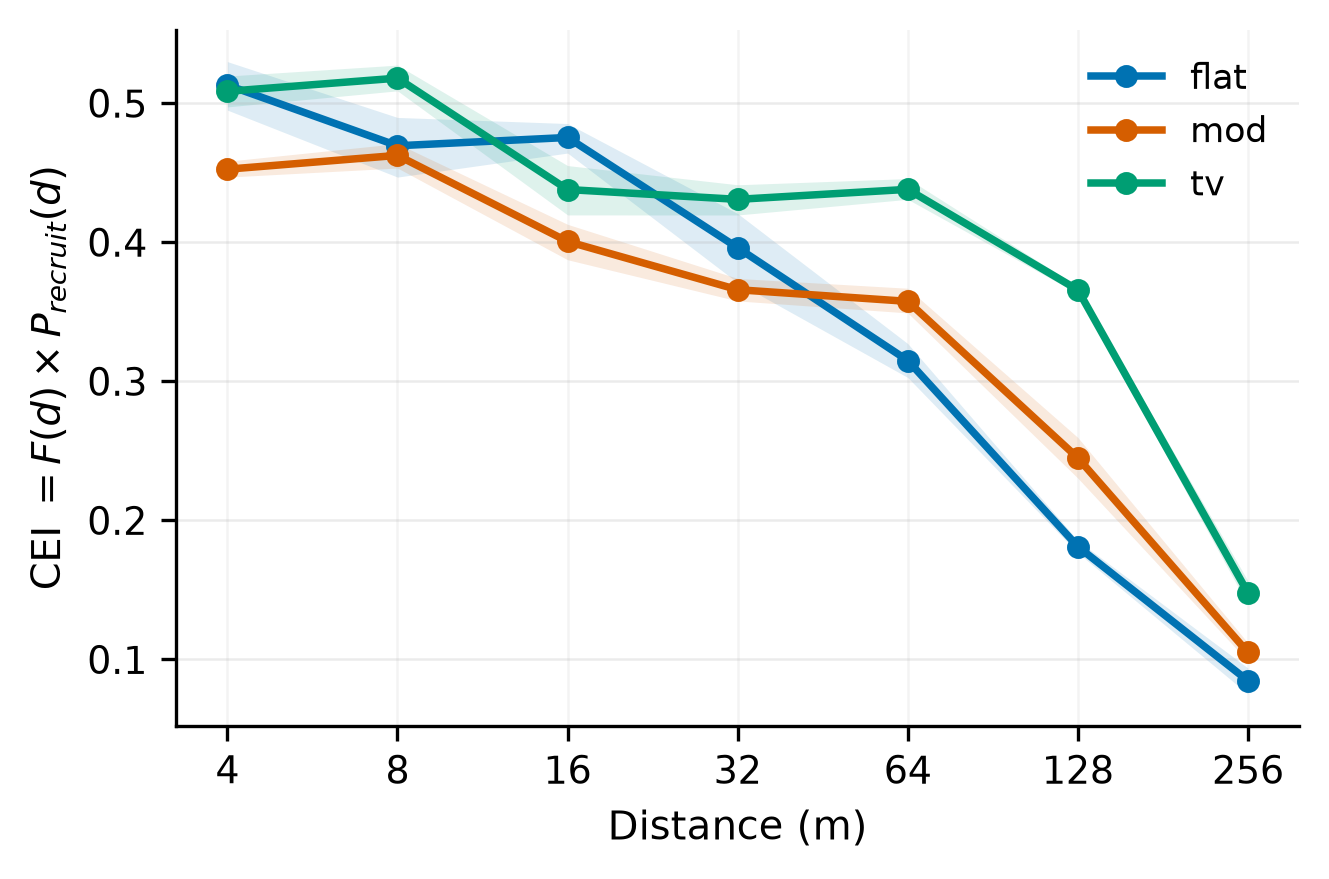
\includegraphics[width=0.42\textwidth]{figs/fig7_cei.png}
  \caption{Communication effectiveness index against distance. The bands reflect fidelity
  sampling only (block bootstrap over the 30 blocks); the recruitment term is held at its point
  estimate. The index is not monotone over 4--64 m because the fidelity curves themselves are
  not.}\label{fig:q4-cei}
\end{figure}

\subsection{Expected number of responders}\label{sec:q4-expected}

The second output the problem permits is the expected number of responding individuals. Let
$p(n)$ be the empirical distribution of group size (139 experiments; median 8, interquartile
range 3--15, mean 10.75, maximum 40). Then
\begin{equation}\label{eq:expected}
  \E[N_{\mathrm{resp}}\mid d] \;=\; \rho \sum_{n} p(n)\; n\; \Prob(\text{any}\mid n,d),
\end{equation}
where $\rho$ is the fraction of individuals in a responding group that actually participate.
The probability in Equation~\eqref{eq:expected} is the probability of \emph{any} response, not
$P_{\mathrm{recruit}}$: the two outputs answer different questions. The index asks how strong the
communication channel is and uses the narrower recruitment event (approach or vocalisation),
whereas the expected-responder count asks how many birds arrive and therefore keeps the broader
any-response event. The
data contain no individual marks, so $\rho$ is not identifiable and is treated as a sensitivity
parameter rather than estimated.

\begin{table}[htbp]
  \centering
  \caption{Expected number of responders by distance and call type, for $\rho=1$ and $\rho=0.5$.}\label{tab:q4-expected}
  \small
  \begin{tabular}{lrrrrrr}
    \toprule
    & \multicolumn{3}{c}{$\rho = 1$} & \multicolumn{3}{c}{$\rho = 0.5$} \\
    \cmidrule(lr){2-4}\cmidrule(lr){5-7}
    Distance (m) & flat & mod & tv & flat & mod & tv \\
    \midrule
    4 & 8.78 & 9.02 & 9.41 & 4.39 & 4.51 & 4.71 \\
    50 & 5.03 & 5.44 & 6.20 & 2.51 & 2.72 & 3.10 \\
    100 & 3.87 & 4.26 & 5.01 & 1.93 & 2.13 & 2.51 \\
    150 & 3.24 & 3.60 & 4.33 & 1.62 & 1.80 & 2.16 \\
    256 & 2.50 & 2.81 & 3.47 & 1.25 & 1.41 & 1.73 \\
    \bottomrule
  \end{tabular}
\end{table}

Because $\rho$ enters linearly it scales every entry of Table~\ref{tab:q4-expected} without
changing the ordering of call types. Sweeping it over the full range requested by the problem,
from 0.1 to 1.0, gives at 100 m the triplets (0.39, 0.43, 0.50) at $\rho=0.1$, (1.93, 2.13, 2.51)
at $\rho=0.5$ and (3.87, 4.26, 5.01) at $\rho=1$. The ratio between call types is invariant by
construction, which is the point: the one parameter we cannot estimate cannot explain away the
difference between the call types.

\subsection{Scenarios and sensitivity}\label{sec:q4-sens}

Table~\ref{tab:q4-scen} and Figure~\ref{fig:q4-scen} report a baseline plus six
perturbations: two thresholds taken from the problem's examples (0.5 to 0.6 and 0.7), two
reductions in all three correlations (5 and 20 percentage points), a 3 dB noise increase, and one
impairment of recruitment (implemented as a deterioration of sea state).

\begin{table}[htbp]
  \centering
  \caption{Behaviour-limited radius (m) under seven scenarios.}\label{tab:q4-scen}
  \small
  \begin{tabular}{lrrr}
    \toprule
    Scenario & flat & mod & tv \\
    \midrule
    Baseline & 136.6 & 174.8 & 203.4 \\
    Recognition threshold 0.6 & 102.4 & 141.1 & 170.8 \\
    Recognition threshold 0.7 & 77.8 & 109.1 & 143.3 \\
    Correlations $-5$ percentage points & 128.3 & 166.8 & 196.2 \\
    Correlations $-20$ percentage points & 107.1 & 140.3 & 171.0 \\
    Noise $+3$ dB (fidelity $-0.10$) & 102.4 & 141.1 & 170.8 \\
    Sea state (recruitment $\times0.8$) & 107.1 & 140.3 & 171.0 \\
    \bottomrule
  \end{tabular}
\end{table}

\begin{figure}[htbp]
  \centering
  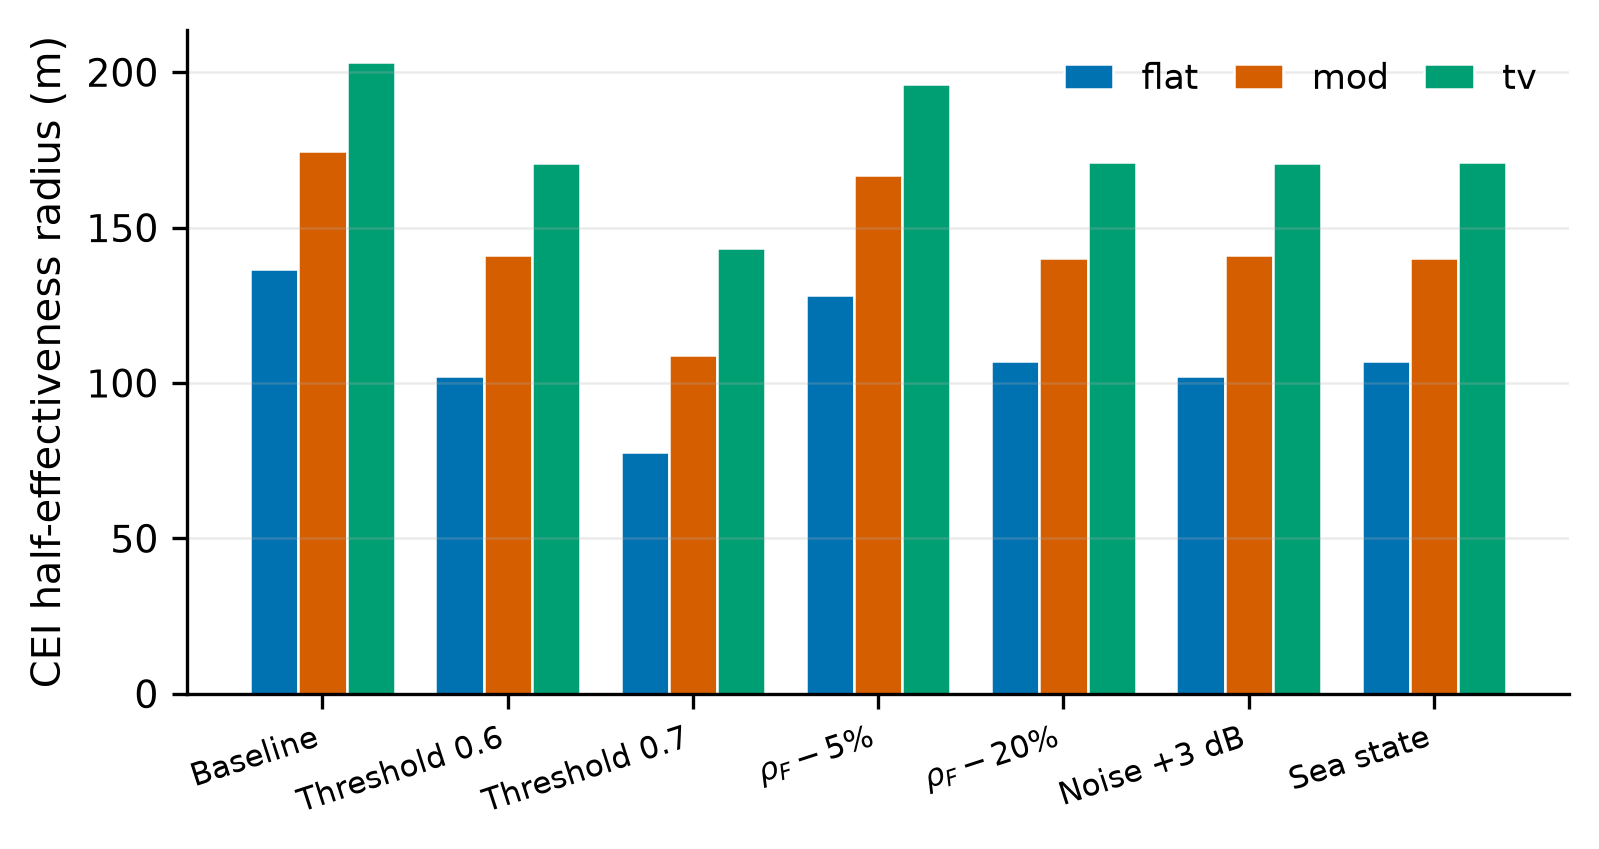
\includegraphics[width=0.52\textwidth]{figs/fig8_scenarios.png}
  \caption{Behaviour-limited radii under the seven scenarios of Table~\ref{tab:q4-scen}.}\label{fig:q4-scen}
\end{figure}

Three results stand out. First, the threshold is the most consequential single choice: moving from
0.5 to 0.7 shortens the two-voice radius from 203 to 143 m, a 30\% reduction. Second, the ranking
of call types is stable across the seven rows --- two-voice remains first and flat last.
The exception to this stability does not appear in the table: it appears in the weight
sensitivity of Section~\ref{sec:q2-sens}, where an envelope-heavy weighting reverses the order.
Third, two pairs of rows are numerically identical by construction. Threshold 0.6 and the 3 dB
noise scenario coincide because both were implemented as a shift of $-0.10$ in fidelity, and the
$-20$ percentage-point correlation reduction coincides with the sea-state scenario because both
were implemented as a multiplication of the index by 0.8. These are limitations of a
one-dimensional scenario design, not coincidences in the data; a finer noise model would require
an explicit signal-to-noise calculation that the supplied data do not support.

The exception is the envelope weight. If the envelope correlation is given weight 0.5 instead of
one third, the two-voice radius at $\tau=0.7$ collapses to 12.1 m while the modulated radius
remains at 66.8 m. The reason is that the two-voice envelope correlation is the lowest of the
three call types at 256 m (0.139), even though its spectrogram correlation is the highest. The
statement ``two-voice calls travel furthest'' is therefore true for the spectral metrics and false
for the envelope metric, and the equal-weight index sits between the two. This is the single
largest structural uncertainty in the analysis, and it is why Section~\ref{sec:discussion}
reports a range rather than a number.

\subsection{Conservation recommendations}\label{sec:q4-rec}

The index translates into four concrete recommendations and one caveat.

\begin{enumerate}[leftmargin=1.8em,itemsep=3pt]
  \item \textbf{A 200 m noise-management buffer around foraging hotspots.} The behaviour-limited
        half-effectiveness radius of the two-voice call is 203 m on the empirical curve and 158 m
        under a logistic fit. A 200 m buffer approximately covers the empirical estimate (203 m); a precautionary
        manager who prefers the conservative estimate would choose 160 m. We recommend 200 m as
        the primary figure and state the 160 m alternative explicitly.
  \item \textbf{A 3 dB limit on vessel noise in the 0.5--2 kHz band.} The first fundamental of
        all three call types lies between 221 and 334 Hz, and the 75th percentile of the spectral
        energy lies near 1.1 kHz, so the 0.5--2 kHz octave band carries most of the signal energy
        as well as most of the engine noise. A 3 dB increase in that band shortens the effective
        radius to 102--171 m (Table~\ref{tab:q4-scen}), if a 3 dB increase were equivalent to the
        assumed 0.10 drop in fidelity used to build that scenario.
  \item \textbf{Seasonal and diurnal timing.} The playback data were collected in a single season
        and do not identify a diel pattern; we therefore recommend that any restriction be
        evaluated against a monitoring series before being made permanent.
  \item \textbf{Monitoring metric.} The spectrogram correlation of two-voice calls at 128 m
        (0.740) is the most sensitive of the available indicators to long-range change, and it is
        the one we recommend for tracking. The envelope correlation should not be used as the
        primary indicator, because it is both the most variable and the least favourable to the
        two-voice call.
\end{enumerate}

The caveat is that all of these numbers come from a single site, a single season and 139 paired
trials. They are precautionary recommendations, not causal guarantees: a buffer derived from
this index is expected to preserve the \emph{opportunity} for acoustic contact, not to guarantee
that recruitment succeeds.

\section{Uncertainty, robustness and limitations}\label{sec:discussion}

\subsection{Four layers of uncertainty}

The intervals reported in Sections~\ref{sec:q3} and~\ref{sec:q4} are the narrowest of the four
layers of uncertainty that the analysis contains. Reporting them alone would give a false sense
of precision.

\begin{table}[htbp]
  \centering
  \caption{Four layers of uncertainty, their typical magnitude, and how they were handled.}\label{tab:uncertainty}
  \small
  \begin{tabular}{p{2.6cm}p{4.6cm}p{5.6cm}}
    \toprule
    Layer & Magnitude & Treatment \\
    \midrule
    Sampling (blocks) & two-voice radius $\pm 5$ m by block bootstrap & block bootstrap over 30 blocks, not rows \\
    Model family & two-voice radius 158--203 m (logistic vs empirical) & report the range, do not choose \\
    Threshold and weights & radius 203 $\to$ 143 m when $\tau$ moves 0.5 $\to$ 0.7; 12--67 m under envelope weight 0.5 & full sensitivity table, Section~\ref{sec:q4-sens} \\
    Definition of outcomes & any response (all 278 rows) 108 $\to$ 112 across S1--S3 & definitional sensitivity, Table~\ref{tab:defsens} \\
    \bottomrule
  \end{tabular}
\end{table}

The ordering is instructive: the sampling layer, the only one that conventional statistics
reports, is smaller than the others by an order of magnitude. A paper that reported
$203.4\pm5$ m and stopped would be technically correct and practically misleading.

\subsection{What would change the conclusions}

Three statements survive every sensitivity analysis and three do not.

\emph{Robust.} (i) Natural calls elicit far more responses than controls, by a factor between 13
and 37 depending on the matching used. (ii) Response probability declines with distance and with
group size. (iii) The distribution of response combinations differs between call and control.

\emph{Fragile.} (i) The ordering of call types at the 0.5 threshold is model-dependent: a
four-parameter Weibull places modulated marginally ahead of two-voice, while the empirical curve,
the GAM and the three-parameter Weibull place two-voice ahead. (ii) The claim that two-voice
calls are most robust at long range holds for the spectrogram and amplitude-spectrum metrics and
reverses for the envelope metric at 256 m. (iii) The apparent effect of context disappears after
adjustment for group size, and the data cannot say whether the remaining association with group
size is behavioural or observational.

\subsection{Limitations}

\textbf{The observation window is not recorded (L1).} We assume $W=60$ s because it is the upper
bound of the duration field and exceeds the largest observed latency; the sensitivity over 48,
90 and 120 s bounds the effect, and if the true window were shorter some non-responders would be
misclassified. \textbf{Nine zero latencies are excluded from the latency model (L2)}; they are
immediate responses at the resolution of the protocol and would form a point mass that a
continuous likelihood cannot accommodate. \textbf{Playback and propagation trials cannot be
linked (L3)}, because no recording identifier connects them, so $q(d)$ in
Equation~\eqref{eq:decomp} must be imported rather than estimated. \textbf{Date is confounded
with call type (L4)}: the association is strong (Cram\'er's $V=0.528$), and a date-fixed-effects
fit raises the modulated and two-voice odds ratios to about 46 and 39; although the intervals
widen (13--163 and 13--116), both remain significant, so the association survives the date
confound. The estimates are imprecise because date and call type are strongly associated. We keep
the unadjusted model as primary and report the adjusted direction as a caveat. \textbf{The propagation data have a small effective sample (L5)}: thirty
blocks support about 46 effective observations per distance, which the block bootstrap reflects
but cannot enlarge. Finally, \textbf{all conclusions are conditional on a single site and a
single season (L6)} and should not be extrapolated without re-estimation.
\textbf{Recruitment is extrapolated beyond the playback range (L7)}: playback distances stop at
200 m, whereas the CEI curve is evaluated to 256 m, so the two-voice radius of 203 m sits at the
edge of the observed range and should be read as an upper bound of about 200 m. \textbf{The CEI
bands reflect fidelity sampling only (L8)}: the block bootstrap resamples the 30 propagation
blocks but does not propagate the uncertainty in the GEE coefficients for $P_{\mathrm{recruit}}$,
so the bands in Figure~\ref{fig:q4-cei} understate the total uncertainty.

\subsection{Strengths and weaknesses of the model}

The strength of the approach is that it uses the design the data actually have: the pairing is
exploited rather than discarded, censoring is modelled rather than deleted, the block structure
of the propagation data is respected in the CEI intervals of Section~\ref{sec:q4}, and the index
is built from two separately estimated components whose provenance is traceable.

The weakness is that the two components are measured on different scales. Fidelity is a
correlation between waveforms, recruitment is a probability of behaviour, and their product is
dimensionless but not calibrated to any ecological outcome. The index orders distances and call
types correctly; it does not tell us how many calories a bird saves, or how many recruits a
colony needs. Closing that gap would require a fitness-linked experiment that the present data
cannot supply.

\section{Conclusions}\label{sec:conclusion}

\subsection{Answers to the four questions}

\textbf{What distinguishes the three call types?} They differ along the frequency axis, not in
duration or bandwidth. Peak frequency separates the groups after correction ($H=12.28$,
$p=0.013$), and the median first fundamental decreases from flat (298 Hz) through modulated
(287 Hz) to two-voice (274.5 Hz). The two-voice call additionally carries a second fundamental,
which is a structural feature rather than a continuous measurement. A classifier using only the
shared continuous features reaches a macro-$F_1$ of 0.458; admitting the structural indicators
raises it to 0.952, but that gain reflects the definition of the call types, not a better
acoustic description.

\textbf{How far does the signal travel?} Fidelity is nearly constant to 32 m and collapses
between 64 and 256 m. At the operational threshold $\tau=0.5$ the effective ranges are 84.7 m
(flat), 144.6 m (modulated) and 169.7 m (two-voice). The ordering is robust across thresholds and
across most weightings, but not under an envelope-heavy weighting --- at $\tau=0.7$ with weight
0.5 on the envelope correlation the two-voice radius collapses to 12.1 m --- nor across model
families: at $\tau=0.5$ a four-parameter Weibull reverses the modulated and two-voice order. The
three correlations are not independent evidence; the spectrogram and amplitude-spectrum metrics
are strongly correlated (per-type $r=0.81$--$0.97$).

\textbf{Do penguins respond, and to what?} Yes, strongly, and the paired design is what makes
this visible: 64.8\% against 12.9\%, McNemar OR 37.0 (95\% CI 9.9--311). Response declines with
distance (OR 0.49 per $e$-fold) and with group size (OR 0.94 per bird), and the three call types
differ from control (OR 13.7--22.4) but not clearly from one another. The distribution of the
eight response combinations changes under playback ($p=0.0002$); whether call type shifts the
probability of a specific combination is not established ($p=0.137$, 58\% of expected counts
below five). Time to first response has a conditional median of about 2 s and lengthens by a
factor of 1.27 per $e$-fold of distance.

\textbf{What is the communication-effective range?} With
$\mathrm{CEI}(d)=F(d)\times P_{\mathrm{recruit}}(d)$, the behaviour-limited half-effectiveness
radii are 137 m (flat), 175 m (modulated) and 203 m (two-voice) on the empirical curve, with the
two-voice value falling to 158 m under a logistic fit. Recruitment probability itself declines
only weakly with distance (OR 0.87 per $e$-fold, $p=0.59$), so the radius is driven mainly by
fidelity rather than by a behavioural gradient. If a 3 dB increase were equivalent to the assumed
0.10 drop in fidelity, the radii would fall to 102, 141 and 171 m. We translate these into a
precautionary 200 m buffer with a 3 dB limit in the 0.5--2 kHz band.

\subsection{Future work}

Three extensions would materially improve the conclusions. First, recording the observation
window explicitly would turn $W=60$ s from an assumption into a measurement. Second, marking
individual birds would make $\rho$ identifiable and would separate group-level from
individual-level response. Third, an experiment that links a playback trial to a propagation
measurement of the same call would make the perception term $q(d)$ estimable rather than
imported, and would close the largest gap in the present analysis.


\footnotesize
\begin{thebibliography}{9}
\bibitem{ref1} Pichegru, L., et al. (2012). Behavioural inertia places a top marine predator at
risk from environmental change. \textit{Marine Biology}, 159: 1191--1200.
\bibitem{ref2} Favaro, L., et al. (2016). Vocal individuality cues in the African penguin
(\textit{Spheniscus demersus}). \textit{Bioacoustics}, 25(2): 155--171.
\bibitem{ref3} Thiebault, A., et al. (2019). Seabird acoustic communication at sea: a new
perspective using bio-logging. \textit{Scientific Reports}, 9: 12445.
\bibitem{ref4} Liang, K.-Y., Zeger, S. L. (1986). Longitudinal data analysis using generalized
linear models. \textit{Biometrika}, 73(1): 13--22.
\bibitem{ref5} McNemar, Q. (1947). Note on the sampling error of the difference between
correlated proportions or percentages. \textit{Psychometrika}, 12(2): 153--157.
\bibitem{ref6} Stuart, A. (1955). A test for homogeneity of the marginal distributions in a two-way
classification. \textit{Biometrika}, 42(3/4): 412--416.
\bibitem{ref7} Efron, B., Tibshirani, R. (1994). \textit{An Introduction to the Bootstrap}.
Chapman \& Hall/CRC.
\bibitem{ref8} Royston, P., Parmar, M. K. B. (2013). Restricted mean survival time: an
alternative to the hazard ratio. \textit{BMC Medical Research Methodology}, 13: 152.
\end{thebibliography}

\newpage
\appendix
\section{Reproducibility and data availability}
\subsection*{A.1 Reproduction}

All results are deterministic given the seeds. The pipeline has three scripts.

\begin{enumerate}[leftmargin=1.8em,itemsep=2pt]
  \item \texttt{q1\_q2.py} --- descriptive statistics, Kruskal--Wallis and Mann--Whitney tests
        with Holm correction, repeated stratified five-fold cross-validation, date-holdout
        validation, composite fidelity, monotone fitting, bootstrap intervals and the Weibull
        comparisons of Problem~2. Seed 2026.
  \item \texttt{generate.py} --- paired McNemar tests, GEE models, the eight-combination
        permutation test, the two-part AFT model, the nine-row prediction table, CEI curves and
        radii, expected responders and the scenario analysis. Block bootstrap: 2000 resamples of
        the 30 blocks; combination permutation: 5000 swaps.
  \item \texttt{make\_figs.py} --- the eight figures.
\end{enumerate}

Environment: Python 3.14 with numpy 2.5, pandas 3.0, matplotlib 3.11 and statsmodels for the GEE
and AFT fits; XeLaTeX for typesetting. Total runtime under five minutes.

\subsection*{A.2 Data and code availability}

The data are those distributed with the 2026 APMCM Problem C and archived by the problem setters
in the public Zenodo record cited in the problem statement (Data01--11 and Supplementary~1--5).
No external data were used. The three scripts above read only the nine correlation files, Data01
and Data02 from the supplied archive; they, together with the intermediate result tables, are
provided as supplementary material, so every number in this paper can be regenerated exactly.


\subsection*{A.3 Date-adjusted sensitivity for the call-type effect}

Date is strongly associated with call type (Cram\'er's $V=0.528$), so the call-type odds ratios
could in principle be an artefact of when each call type was played. Table~\ref{tab:date-adj}
refits the model of Equation~\eqref{eq:gee} with a fixed effect for each recording date
(12 levels, 19 parameters, 139 clusters).

\begin{table}[htbp]
  \centering
  \caption{Call-type odds ratios before and after adjusting for recording date.}\label{tab:date-adj}
  \small
  \begin{tabular}{lrrrr}
    \toprule
    & \multicolumn{2}{c}{Unadjusted} & \multicolumn{2}{c}{Date-adjusted} \\
    \cmidrule(lr){2-3}\cmidrule(lr){4-5}
    Call type & OR [95\% CI] & $p$ & OR [95\% CI] & $p$ \\
    \midrule
    flat & 13.75 [6.58, 28.73] & $<0.001$ & 15.79 [6.44, 38.73] & $<0.001$ \\
    mod & 16.28 [6.39, 41.47] & $<0.001$ & 45.98 [13.13, 161.07] & $<0.001$ \\
    tv & 22.38 [9.47, 52.89] & $<0.001$ & 38.73 [12.90, 116.26] & $<0.001$ \\
    \bottomrule
  \end{tabular}
\end{table}

Adjustment increases the modulated and two-voice odds ratios by a factor of two to three and
widens their intervals substantially, but every effect remains significant. The date-confound
therefore inflates our uncertainty rather than explaining the effect away.

\subsection*{A.4 The recruitment model behind the index}

The index of Equation~\eqref{eq:cei} uses a second response definition, recruitment
(approach or vocalisation), fitted with the same estimating equations. Table~\ref{tab:gee-recruit}
reports it. Its most important entry is the distance term.

\begin{table}[htbp]
  \centering
  \caption{GEE for recruitment (approach or vocalisation). n = 278, 139 clusters.}\label{tab:gee-recruit}
  \small
  \begin{tabular}{lrrr}
    \toprule
    Term & OR & 95\% CI & $p$ \\
    \midrule
    flat vs control & 54.66 & 16.32--183.07 & $<0.001$ \\
    mod vs control & 42.59 & 13.08--138.63 & $<0.001$ \\
    tv vs control & 68.04 & 20.46--226.23 & $<0.001$ \\
    $\log$ distance (per $e$-fold) & 0.873 & 0.529--1.439 & 0.593 \\
    Group size (per bird) & 0.944 & 0.898--0.992 & 0.023 \\
    Context: commuting vs after & 0.794 & 0.340--1.857 & 0.595 \\
    Context: searching vs after & 2.677 & 0.891--8.044 & 0.079 \\
    \bottomrule
  \end{tabular}
\end{table}

Recruitment declines only weakly with distance and not significantly ($p=0.59$), whereas the
any-response outcome of Table~\ref{tab:q3-gee} declines clearly ($p=0.008$). The difference is
informative: distance mainly suppresses the cheap responses (heads-up, vocalisation) rather than
the decision to approach. It also means that the distance profile of the index is driven by
fidelity rather than by behaviour.

\subsection*{A.5 Software and source code}

Software: Python 3.14 with numpy 2.5, pandas 3.0, matplotlib 3.11 and statsmodels 0.15;
XeLaTeX for typesetting.

The complete source code is provided in the supplementary archive submitted with this paper
(\texttt{Capmcm26XXXXXXfj.zip}), as required by the submission specification. It consists of
three files, listed here with their size and the results they produce.

\begin{table}[htbp]
  \centering
  \caption{Source files in the supplementary archive.}\label{tab:code}
  \small
  \begin{tabular}{llrl}
    \toprule
    File & Produces & Lines & Random seed \\
    \midrule
    \texttt{q1\_q2.py} & Problem 1 and Problem 2 results, Figures 1--2 & 473 & 2026 \\
    \texttt{generate.py} & Problem 3 and Problem 4 results, Tables 8--22 & 391 & fixed \\
    \texttt{make\_figs.py} & Figures 1--8 & 232 & fixed \\
    \bottomrule
  \end{tabular}
\end{table}

The scripts read only the data files distributed with the problem and write plain CSV tables, so
every number in this paper can be regenerated without any private dependency. The code is not
reproduced in the appendix because its string literals contain the Chinese names of the output
tables, which would violate the English-only requirement for the paper.


\end{document}
